\documentclass[a4paper,10pt]{article}

\author{Santiago Domínguez Collado}
\title{Borrador TFG}
\usepackage{titlesec}

\setcounter{secnumdepth}{4}

\titleformat{\paragraph}
{\normalfont\normalsize\bfseries}{\theparagraph}{1em}{}
\titlespacing*{\paragraph}
{0pt}{3.25ex plus 1ex minus .2ex}{1.5ex plus .2ex}

\usepackage{lmodern}
\usepackage[T1]{fontenc}
\usepackage[spanish]{babel}
\usepackage[utf8]{inputenc}
\usepackage{mathtools}
\usepackage{ amssymb }
\usepackage{graphicx}
\usepackage[margin=1.50in]{geometry}
\graphicspath{{imagenes/}}
\usepackage{float}
\usepackage{listings}
\newtheorem{theorem}{Teorema}
\newtheorem{proposition}{Proposición}
\newtheorem{definition}{Definición}
\usepackage{float}
\usepackage[none]{hyphenat} %no corta las palabras al compilar el documento
\sloppy %como no se cortan las palabras el texto se descuadra, justifica los p�rrafos
\usepackage{geometry}
\geometry{textwidth=474pt} %Corrige algo de geometry
\begin{document}
\begin{center}
\begin{LARGE}
Machine Learning \\
\vspace*{0.15in}
\UseRawInputEncoding
Borrador TFG
\end{LARGE}
\end{center}
\begin{center}
\begin{large}
Santiago Domínguez
\end{large}
\end{center}


\tableofcontents




\section{Introducción.}
El Aprendizaje Automático (o Machine Learning, ML, en inglés) es la rama de la inteligencia artificial que permite la inferencia de un modelo, de manera autónoma, por parte de un ordenador (Samuel 1959). En la pasada década, el ML ha permitido un espectacular desarrollo de la conducción autónoma (aún en fase experimental), el reconocimiento de voz y escritura manual, la búsqueda efectiva en la web y una vasta mejora del conocimiento del genoma humano. El ML es tan omnipresente que probablemente lo usamos decenas de veces al día sin saberlo. Desde Los sistemas de recomendación de publicidad basados en nuestros clicks en páginas webs hasta el clasificador de spam de nuestra cuenta de correo electrónico usan algoritmos de ML (supervisado, en el segundo caso, no-supervisado en el primero). Y en conexión con áreas de investigación de nuestro departamento, es necesario mencionar el proyecto EMPATIA-BIND, conjunto con la UC3M, de cara a la prevención y combate de a violencia de género, que ha ganado un proyecto europeo recientemente.
El ML se nutre de una importante base de cálculo diferencial, optimización, álgebra lineal y análisis numérico, así como estadística exploratoria, bayesiana y teoría de la probabilidad, y en su parte inferencial, puede tender a solaparse con la estadística, aunque a diferencia de esta, son cruciales el estudio e implementación de algoritmos atendiendo al orden de complejidad y su explotación en plataformas escalables.
\newpage
\section{Machine Learning.}

\subsection{Discusión preliminar.}
\subsection{Base matemática del Machine Learning.}
\label{}

En el presente trabajo, entenderemos por optimización, el cálculo (exacto o
aproximado) de los máximos y/o mínimos de una funcóon en su dominio, si es
que estos existen.\\
En nuestro caso, nos restringiremos a funciones que miden el error entre
un modelo teórico aproximado y una serie de muestras empíricas, cuyo modelo
teórico subyacente pretendemos establecer o aproximar.
\\Nos serviremos de la teoría de la optimización para alcanzar (o aproximar) los valores en los que estas funciones de error alcanzan su mínimo y así obtener el mejor resultado posible de nuestro modelo. Nos referiremos a estos valores como parámetros óptimos.
\subsubsection{Teorema
de Weierstrass y condiciones de primer orden}
Lo primero es estudiar en qué condiciones se alcanzan el máximo y/ o mínimo.
A este respecto, uno de los resultados más importantes es el teorema de Weierstrass, que establece que toda función continua $f$, definida en un dominio cerrado
y acotado alcanza sus valores máximos y mínimos en algún punto del dominio.
Más precisamente:
\begin{theorem}
Sea A un conjunto cerrado y acotado, denotemos por $\mathcal{C}(A,\mathbb{R})$  el conjunto de funciones continuas de $A$ en $\mathbb{R}$ entonces existen $ x_{1},x_{2} \in A$, tales que $ f(x_{1}) \leq f(x) \leq f(x_{2})$ para todo valor de $x$ en $A$.
\end{theorem}
\noindent
Una vez sabemos que se alcanzan los extremos, veamos cómo calcularlos.
\\Sea $A$ un subconjunto de $\mathbb{R}^n$ y denotemos por $\mathring{A}$ en interior de $A$, es decir, el mayor conjunto abierto contenido en A.
\begin{definition}
(Máximo relativo). Se dice que la función $f$ definida en un conjunto $D\subseteq \mathbb{R}^n$ tiene un valor máximo local o relativo en un punto $c\in\mathring{D}$, si $f(c)\geq f(x)$ para todo $x$ perteneciente a un entorno de $c$. El valor máximo relativo de $f$ correspondiente a $c$ es $d = f(c)$.
\end{definition}
\begin{definition}
(Mínimo relativo). Se dice que la función $f$ definida en un conjunto $D\subseteq \mathbb{R}^n$ tiene un valor mínimo local o relativo en un punto $c\in\mathring{D}$, si $f(c)\leq f(x)$ para todo $x$ perteneciente a un entorno de $c$. El valor mínimo relativo de $f$ correspondiente a $c$ es $d = f(c)$.
\end{definition}
El siguiente resultado es una condición necesaria de primer orden (es decir,
utiliza las primeras derivadas parciales) y cuya demostración se puede ver en
cualquier texto de cálculo en varias variables:

\begin{proposition}
Sea $ f : A \rightarrow \mathbb{R}$ una función continua en $A$ y con derivadas
parciales en todo punto de $\mathring{A}$. Sea $x\in A$ un máximo o mínimo local,
entonces $\nabla f(x)=(0,...,0)$.

\end{proposition}

\subsubsection{Búsqueda de mínimo absoluto.}
Para buscar los extremos de una función f definida en un conjunto $A\subseteq \mathbb{R}^n$, examinamos, por un lado, los
puntos interiores de gradiente cero (extremos relativos, conforme a la proposición
1), los puntos de la frontera, y los puntos interiores sin derivada. 
\\En esta sección utilizaremos la el concepto de matriz definida y semidefinida:
\begin{definition}Sea M una matriz cuadrada con entradas reales.
\begin{itemize}
\item M es definida positiva $\Longleftrightarrow x^TMx \geq 0$ y $x^TMx=0\Leftrightarrow x=0$
\item M es definida negativa  $\Longleftrightarrow x^TMx \leq0$ y $x^TMx=0\Leftrightarrow x=0$
\item M es semidefinida positiva  $\Longleftrightarrow x^TMx \geq0$ para todo $x$.
\item M es semidefinida negativa  $\Longleftrightarrow x^TMx \leq0$  para todo $x$.
\end{itemize}
\end{definition}
\begin{definition}
Matriz Hessiana:  Denotemos por $\mathcal{C}^2(A,\mathbb{R})$  el conjunto de las funciones definidas
sobre $A$, dos veces diferenciables con continuidad, con valores en $\mathbb{R}$ y sea $f \in
C^2(A, \mathbb{R})$. La matriz Hessiana de $f$ en $(x, y) \in A$, se define del siguiente modo:

$$
H_f(x,y)=\left(
\begin{array}{cc}
\frac{\partial^2f}{\partial x^2}(x,y) & \frac{\partial^2f}{\partial y\partial x}(x,y) \\
\frac{\partial^2f}{\partial y\partial x}(x,y) & \frac{\partial^2f}{\partial y^2}(x,y)
\end{array}
\right)
$$
\\
Su determinante $|H_f(x,y)|$ se denomina Hessiano de $f$.
\end{definition}
El siguiente resultado es una condición necesaria de segundo orden, cuya demostración se basa en el criterio de Sylvester y en el desarrollo en serie de Taylor
para funciones de dos variables:
\begin{theorem}
Sea $D\subseteq \mathbb{R}^n$ un conjunto abierto, y $f\in\mathcal{C}^2(D,\mathbb{R})$. Dado un punto $(x_0,y_0)\in D$, se tiene:
\begin{itemize}
    \item Si $\begin{vmatrix}H_f(x_0,y_0)\end{vmatrix}>0$ y $ f_{xx}(x_0,y_0)>0$, entonces $\begin{vmatrix}H_f(x_0,y_0)\end{vmatrix}$ es definida positiva
y $f$ tiene un mínimo relativo estricto en $(x_0, y_0)$.
    \item Si $\begin{vmatrix}H_f(x_0,y_0)\end{vmatrix}>0$ y $ f_{xx}(x_0,y_0)<0$, entonces $\begin{vmatrix}H_f(x_0,y_0)\end{vmatrix}$ es definida negativa
y $f$ tiene un máximo relativo estricto en $(x_0, y_0)$.
    \item Si $\begin{vmatrix}H_f(x_0,y_0)\end{vmatrix}\geq0$ y $ f_{xx}(x_0,y_0)\geq0$, entonces $\begin{vmatrix}H_f(x_0,y_0)\end{vmatrix}$ es semidefinida positiva
y $f$ tiene un mínimo relativo estricto en $(x_0, y_0)$.
  \item Si $\begin{vmatrix}H_f(x_0,y_0)\end{vmatrix}\geq0$ y $ f_{xx}(x_0,y_0)\leq0$, entonces $\begin{vmatrix}H_f(x_0,y_0)\end{vmatrix}$ es semidefinida negativa 
y $f$ tiene un máximo relativo estricto en $(x_0, y_0)$.
\end{itemize}

\end{theorem}
\noindent
Existen diversas formas de evaluar si un extremo relativo es absoluto:

\begin{itemize}
\item El dominio es cerrado y acotado y expresado con restricciones de desigualdad, el algoritmo de Karush-Khun-Tucker suele dar buenos resultados.
\item Si hay restricciones de igualdad, se suele aplicar el algoritmo de multiplicadores de Lagrange
\item Con funciones convexas utilizamos resultados específicos que revisamos a
continuación.

\end{itemize}


\subsubsection{Convexidad.}

El estudio de la convexidad permite evaluar si un extremo relativo es absoluto. Por lo tanto, nos interesa demostrar la convexidad de la función de error para determinar nuestro parámetros óptimos.\\

\begin{definition}(Conjunto convexo). Decimos que un conjunto $D\subseteq \mathbb{R}^n$
es convexo si para todo par de puntos $x,y \in D$, el segmento que los conecta está contenido en D, es decir, si para todo $t\in[0,1],tx+(1-t)y\in D$.
\end{definition}
\begin{definition} (Función convexa). Sea $D\subseteq \mathbb{R}^n$ un conjunto convexo y $f: D\rightarrow \mathbb{R}$ una función continua definida en $D$. Decimos que $f$ es convexa si, para todos $x,y\in D$, se tiene:
\[
f(tx+(1-t)y) \leq tf(x)+(1-t)f(y)
\].
\end{definition}

\begin{proposition}
Sea $D$ un dominio convexo y $f\in\mathcal{C}^2(D,\mathbb{R})$. Dado un punto
$(x_0, y_0) \in D$, si la matriz Hessiana $H_f (x_0, y_0)$ es semidefinida positiva, entonces
$f$ es convexa en un entorno de $(x_0, y_0)$.
\end{proposition}
\noindent
El siguiente resultado es una condición suficiente de extremo global para funciones convexas.
\begin{theorem}
Sea $D\in\mathbb{R}^n$ un conjunto convexo y abierto, y $f\in\mathcal{C}^2(D,\mathbb{R})$ una función convexa. Si $\overline{x}_0=(x_0,y_0)\in D$ es un mínimo local, entonces es también el único mínimo global. En particular, si $H_f(x_0,y_0)$ es semidefinida positiva, entonces, $(x_0,y_0)$ es el único mínimo global.
\end{theorem}
\newpage
\section{Regresión lineal}

Sea un conjunto de datos $(x_i,y_i)^n_{i=1}$, queremos obtener la recta que mejor se ajuste a la nube de puntos. Esta recta tendrá la forma $h_\theta(x)= ax+b$ (puede tener  más parámetros). Es decir, debemos escoger$  (a,b)\in \mathbb{R}^2 $ tal que $\text{EMC(a,b)} = \frac{1}{N} \sum_{i=1}^{N}(y_{i}-ax_{i}-b)^2 \text{mínimo.} $



\subsection{Cálculo de mínimos y máximos locales:}
A continuación, mediante el gradiente, probamos que la función ECM tiene
un único extremo local, y mediante la matriz Hessiana, probamos que este es un
mínimo local, y que al ser esta matriz semidefinida positiva, la función ECM es
convexa y el mínimo global es el único mínimo global.
\[\frac{\partial{H}}{\partial{b}}=-2\sum_{i=1}^{N}y_{i}-ax_{i}-b=0\Rightarrow \sum_{i=1}^{N}ax_{i}+bN=\sum_{i=1}^{N}y_{i}\Rightarrow b=\Bar{y}-a\Bar{x}\]
\[\frac{\partial{H}}{\partial{a}}=-2\sum_{i=1}^{N}(y_{i}-ax_{i}-b)x_{i}=0\Rightarrow \sum_{i=1}^{N}x_{i}y_{i}=a\sum_{i=1}^{N}x_{i}^2+b\sum_{i=1}^{N}x_{i}\Rightarrow a \frac{1}{N}\sum_{i=1}^{N}x_{i}^2+(\Bar{y}-a\Bar{x})\Bar{x}=\sum_{i=1}^{N}x_{i}y_{i}\Rightarrow\] 
\[\Rightarrow a[ \,\frac{1}{N} \sum_{i=1}^{N} x_{i}^2-\Bar{x}^2] \,+\Bar{y}\Bar{x}=\frac{1}{N}\sum_{i=1}^{N}x_{i}y_{i}\Rightarrow a\partial_x^2=s_{xy}\Rightarrow\]
\[\boxed{a=\frac{s_{xy}}{\partial_{x^2}}, b=\Bar{y}-\frac{s_{xy}}{\partial_{x^2}}\Bar{x}}\]
\\
\\A continuación, calculamos la matriz Hessiana.\\
$H_f(a,b)$: $
\begin{bmatrix}
    \frac{\partial^2 H}{\partial a^2} & \frac{\partial^2 H}{\partial a \partial b} \\
    \frac{\partial^2 H}{\partial a \partial b} & \frac{\partial^2 H}{\partial a^2}
\end{bmatrix} $\\
Basta con que la matriz sea semidefinida positiva.para ello, observamos que $\frac{\partial^2 E}{\partial a^2}= 2 \sum_{i=1}^n x_{i}^2\leq 0$ y que
$$
|H_f(a,b)|=4\left(\frac{2}{N}\sum_{i_1}^N x_i^2-\overline{x}^2\right)=4\left(\frac{1}{N}\sum_{i_1}^N x_i^2+s_x^2\right)\geq 0,
$$
\subsection{Regresión lineal multivariable.}

El estudio regresión lineal multivariable se utiliza para hallar, si la hay, la relación entre múltiples variables con su salida, con el objetivo de formular una hipótesis que será útil para predecir futuros resultados con nuevas entradas. \\
Supongamos que tenemos las siguientes entradas y salidas: 

\begin{figure}[H]
\centering
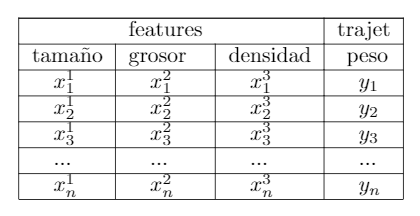
\includegraphics[scale=0.7]{Annotation 2020-03-23 133547}
\end{figure}
 \[\text{En este caso, el error cuadrático medio es } E(a_{1},a_{2},a_{3},a_{4})=\frac{1}{N}\sum_{i=1}^{N}(a_{1}x_i^1+a_{2}x_i^1+a_{3}x_i^1+a_{4}-y_{i})^2
\]
\\Procedemos a calcular el mínimo de los coeficientes que acompañan a las variables de problema, es decir, el mínimo de $\vec{a}$.
\indent
\\Consideremos las matrices:
\[X= \begin{bmatrix}
    x_{1}^1 & x_{1}^2 & x_{1}^3 & x_{1}^4  \\
    .&.&.&.\\
    .&.&.&.\\
    .&.&.&.\\
    x_{N}^1 & x_{N}^2 & x_{N}^3 & x_{N}^4 
\end{bmatrix} \in M_{M*n}. \hspace{0.20cm} y=\begin{bmatrix}y_{1}\\y_{2}\\.\\.\\.\\y_{N}\end{bmatrix}\] \\ \[E(\vec{a},b)=||X\vec{a}-y||^2 = <x\vec{a}-\vec{y},x\vec{a}-y>=<x\vec{a},x\vec{a}>-2<X\vec{a},y>+<y,y>\]
\[\nabla E(a)=\nabla<x\vec{a},x\vec{a}>-2\nabla<x\vec{a},\vec{y}>=0\Leftrightarrow \boxed{ \vec{a}=(X^T X)^{-1} X^T y}\]
Al igual que en la Regresión Lineal univariable, se demuestra que la función EMC es convexa, por lo tanto $\vec{a}$ es un mínimo global.


\subsection{Método iterativo.}

El anterior método explicado en el apartado de regresión lineal multivariable muestra cómo obtener la hipótesis de forma directa, analítica, no obstante, en la realidad, el cálculo de la inversa de una matriz se evita en la mayoría de las ocasiones debido a la complejidad que esta requiere: O($n^3$).\\
En su lugar, métodos iterativos como gradient descent, el cual “desciende” por la función de error gracias al cálculo constante de los parámetros en cada iteración, muestran una complejidad inferior O($n^2$), la cual es viable computacionalmente para trabajar. 

\subsection{Algoritmo Gradient Descent.}
El algoritmo gradient descent es uno de los algoritmos de optimización más populares en el ML. Se utiliza para minimizar una función $J$  moviéndose de forma iterativa en la dirección del gradiente de dicha función. Dicha función es conocida como función de coste. 
\\En cada iteración se recalcula el gradiente y se actualiza la aproximación de
los parámetros.
El intervalo que "descendemos" \hspace{0.16cm}por el gradiente está condicionado por la variable learning rate. \\Con un alto learning rate descenderemos más rápido, arriesgándonos a ignorar el mínimo de la función.\\ Con un learning rate muy bajo tendremos que recalcular el gradiente numerosas veces, probablemente sin hallar un resultado óptimo en un tiempo aceptable.
\begin{figure}[H]
\centering
\includegraphics[scale=0.6]{Annotation 2020-05-12 182629.png}
\end{figure}

Durante el desarrollo de este trabajo utilizaremos este algoritmo en el ámbito de las redes neuronales, explicando la forma en la que se lleva a la práctica.

\subsection{Regresión polinomial.}

Cuando nuestra nube de puntos no se ajusta a una línea recta, la regresión lineal no nos sirve para definir una hipótesis que se ajuste a nuestro modelo de datos.
\begin{figure}[H]
\centering
\includegraphics[scale=1.0]{Annotation 2020-05-09 115847.png}
\end{figure}
En tal caso recurrimos a la regresión no lineal. Esta abarca diversos modelos, los más utilizados son: regresión exponencial, regresión potencial, regresión logarítmica y regresión polinomial. Se utiliza cada modelo cuando el conjunto de
datos tiende a ajustarse por una curva respectivamente exponencial, potencial,
logarítmica o polinomial. Nosotros nos ocuparemos sólo de la regresión polinomial.\\
Comencemos por el modelo más sencillo (regresión cuadrática):
\[
 y=\theta_0+\theta_1 x+\theta_2 x^2
\]
Se trata, como antes, de resolver el problema:
\[
 min\sum_{i=1}^{N}(y-\theta_0-\theta_1 x-\theta_2 x^2)^2\longrightarrow \hat{\theta_0},\hat{\theta_1},\hat{\theta_2}
\] 
\begin{figure}[H]
\centering
\includegraphics[scale=1.0]{Annotation 2020-05-09 120107.png}
\end{figure}
Podríamos considerar una hipótesis más ambiciosa como $y=\theta_0+\theta_1 x+\theta_2 x^2 ...\hspace{0.15cm} \theta_20 x^n$ pero esto nos podrá llevar a un ajuste de nuestro modelo demasiado preciso como para funcionar correctamente con datos de prueba. Esto se conoce como \textit{Overfitting} o \textit{Variance problem}.
\\Eso nos lleva al problema de determinar el número de parámetros del modelo. Necesitamos saber cómo aplicar regresión polinomial, en qué grado.
\subsection{Lineal vs polinomial.}

En la práctica, la decisión de aplicar regresión lineal o polinomial puede no ser algo trivial, por ello, antes de reflexionar sobre el número de parámetros que queremos aplicar a nuestro modelo, debemos primero, determinar si la naturaleza del problema corresponde a un problema polinomial, o si por el contrario, la regresión lineal es suficiente para abordarlo.
\subsubsection{Coeficiente de Pearson.}

El coeficiente de correlación lineal de Pearson ($r_{xy}$) nos sirve para determiar la naturaleza de la relación que guardan los datos entre sí. \\El coeficiente se comprende entre 1 y -1, cuanto más cercano está a ±1 más aconsejable será aplicar regresión lineal.
\[
r_{xy}=\frac{s_{xy}}{s_x s_y}
\]
El coeficiente de Pearson es válido solo cuando se cumplan las siguientes condiciones:
\begin{itemize}
    \item Los datos sean muestras independientes, es decir, no hay autocorrelación entre ellos.
    \item Los errores presenten una distribución normal.
    \item Los errores deben ser homocedásticos: es decir, deben tener la misma
varianza poblacional.
\end{itemize}
\subsubsection{Coeficiente de Spearman.}

El coeficiente de Spearman ($\rho$) es una medida de correlación utilizada en lugar del coeficiente de Pearson, cuando no se cumple algunas de las condiciones mencionadas en el apartado anterior. El resultado de este se interpreta al igual que en el coeficiente de Pearson. \\Si el resultado es cercano 1 ó -1, no es necesario aplicar regresión polinomial.
\[
\rho = 1 - \frac{6\sum D^2}{N(N^2 - 1)}
\]
Siendo $D$  la diferencia entre los correspondientes estadísticos de orden de x - y, y siendo $N$ el número de datos.

\subsubsection{Sobre el término "polinomial".}

\indent
Realmente la distinción entre regresión multivariable y polinomial puede verse reducida a un mero formalismo. La diferencia sustancial radica en que en la regresión polinomial las variables son dependientes entre ellas y eso tiene una implicación crítica: se rompe la convexidad, por lo que el mínimo local puede no ser único, eso se da cuando la matriz de variables no es invertible.
\subsection{Regularización.}

En el ajuste de un modelo polinomial, aplicando la teoría explicada hasta ahora, nos surge la duda de cuál es el grado que mejor resultado nos dará, o dicho de otra forma; ¿Qué grado en nuestro modelo es el que mejor se ajusta a nuestras necesidades?\\ A continuación, explicamos dos posibles problemas que suelen aparecer al estimar el grado por exceso.
o por defecto.\\
\begin{definition}(Bias o sobresimplificación). Se dice que nuestro modelo está
sobresimplificado o tiene problema de bias cuando nuestra hipótesis no se ajusta
correctamente a los datos. También se conoce como \textit{underfitting}.

\end{definition}
\begin{definition}(Variance o sobreajuste). Se dice que nuestro modelo está sobreajustado o tiene problema de variance cuando nuestra hipótesis se ajusta demasiado a los datos de la muestra, siendo solo capaz de predecir correctamente
dichos datos, y no nuevos. Es decir, cuando es incapaz de generalizar. También
se conoce como \textit{overfitting}.


\end{definition}
La técnica de penalización permite penalizar los términos de mayor grado de nuestro modelo, permitiéndonos así utilizar hipótesis de un grado considerable, por lo que no hay lugar a que aparezca el problema de bias, mientras que eludimos el problema de variance. Por ejemplo, consideremos este modelo:
\[
 y=\theta_0+\theta_1 x+\theta_2 x^2+1000\theta_3 x^3+1000\theta_4 x^4 = h_\theta (x)
\]
El hecho de que los parámetros $\theta_3$ y $\theta_4$ aparezcan multiplicados por un término
alto implica que si no son demasiado pequeños, tendrán un alto impacto en el
modelo que debe ajustar la nube de puntos.\\
El anterior ejemplo nos sirve para el caso en el que sabemos qué es lo que hay que penalizar, pero para poder usarlo en un caso general, en el que no conozcamos a priori los elemento a penalizar en nuestra hipótesis, la función de coste utilizada hasta ahora será modificada. Sea $J$ la función de coste:

\[
J(\vec{\theta})=\frac{1}{2m}\left[\sum_{i=1}^{m} \left(h_\theta (x^{(i)})-y^{(i)}\right)-\lambda \sum_{j=1}^{n}\theta_{j}^2\right]
\]
Como vemos, aparece la variable $\lambda$, la cual será definida de forma empírica, una $\lambda$ muy superior a 1, provocaría variance, y si es muy cercana a 0, provocaría bias. Los valores típicos suelen rondar el 0,95.\\
Además de ser una manera eficaz para mejorar nuestro modelo, previniendo dos de los problemas más comunes en el desarrollo del aprendizaje automático. La implementación será tan sencilla como modificar nuestro algoritmo de aprendizaje, modificando todos los términos a partir de $\theta_1$ .\\
\[
\frac{J(\theta)}{\partial\theta_j} = \frac{1}{m} \sum_{i=1}^{m} \left(h_\theta (x^{(i)})-y^{(i)}\right) x_{j}^{(i)}-\frac{\lambda}{m} \sum_{i=1}^{m} \theta_j 
\]

\subsection{Escalamiento de variables (feature scaling).}

Durante el planteamiento del problema a resolver mediante el aprendizaje automático es frecuente encontrarse con diversas variables con distinto rango y dominios. Esto puede causar un aprendizaje más lento, lo que supone más tiempo de entrenamiento para peores resultados. \\
Por ejemplo, en un problema en el que consideramos las variables de temperatura y velocidad del viento para predecir futuras precipitaciones, la $\theta$ correspondiente a  velocidad del viento, al tener valores muy superiores respecto a la temperatura, adquirirá más relevancia para determinar el resultado, aunque en la realidad esto no ocurra.\\ En las redes neuronales, que veremos más adelante, esto se traduce en pesos con una relevancia desorbitada respecto a los demás.\\
Esto se evita escalando las variables para que todas queden con el mismo rango, y a priori, con la misma relevancia:
\[
x_i \longleftarrow \frac{x_i - \overline{x}}{s_i} \epsilon [-1,1]
\]
\hspace{0.20cm}
\[
s_i \hspace{0.20cm} = \  max\hspace{0.20cm}x_{i}^j -min\hspace{0.20cm}x_{i}^j \hspace{0.20cm}
\]
\newpage
\section{Regresión logística.}
En los problemas de clasificación, se busca encontrar un modelo que sea capaz de distinguir diferentes entradas en función de sus características, o dicho de otra forma, que sea capaz de reconocer si un elemento pertenece a una clase u otra. Esto se aplica
en multitud de casos como en la detección de tumores, clasificación de spam,
reconocimiento de dígitos, escritura manual, voz, etc.
 \\Cuando en nuestro problema necesitamos distinguir entre dos clases, estamos hablando de clasificación binaria. En el próximo
capítulo veremos cómo clasificar en varias categorías, utilizando redes neuronales.\\
La regresión logística nos permite establecer un umbral de probabilidad rebasado el cual interpretamos que la variable aleatoria binaria bajo estudio toma el valor
1, en tanto que si no se rebasa, estimaremos que su valor es 0.
\\Observemos que la variable dependiente la podemos interpretar como una etiqueta, que a diferencia de la regresión lineal, adquiere solo dos valores posibles,
y es dependiente de varias características (variables independientes), por lo que
se trata igualmente de un modelo de aprendizaje supervisado.

\begin{figure}[H]
\centering
\includegraphics[width=10.50cm, height=4.5cm]{1_Vd9ZTC1zWJPtV7iXPMJk1Q.png}
\end{figure}
A modo de resumen, enumeramos las propiedades básicas del modelo logístico y lo comparamos con la regresión lineal:

\begin{itemize}
\item Al ser la variable de salida binaria, el problema de clasificación debe de ser binario. Por ejemplo, si queremos distinguir entre si un animal es perro o gato, la regresión logística serviría. Pero no serviría para distinguir imágenes de dígitos en base decimal. Como hemos señalado más arriba, la clasificación en más de dos categorías la abordamos mediante redes neuronales.
\item Como la variable dependiente es en este caso discreta (en particular, es acotada), no se puede proponer sin más un modelo de regresión lineal cuya salida
podamos redondear al entero más próximo. La estrategia sería, esencialmente,
como veremos a continuación, someter una función lineal a lo que interpretaremos como una medida de probabilidad: la función sigmoide. La función lineal
definirá una región umbral tal que si esta se rebasa, estaremos clasificando en la
categoría 1 con una probabilidad prefijada.

\item Como veremos a continuación, en regresión logística, no es fácil a priori utilizar el error cuadrático medio como función de pérdida. Se prefiere, en general,
usar la entropía cruzada, lo que convierte el problema de mínimo en un problema
de máximo. La entropía cruzada se usará también en redes neuronales.

\end{itemize}
La regresión logística es uno de los algoritmos más utilizados en Machine Learning, esto se debe a su gran eficiencia, simplicidad y fácil implementación.\\
El mayor inconveniente de la regresión logística es que solo puede ser utiilizada en problemas de clasificación binaria.

\subsection{La función sigmoide.}
En regresión logística principalmente se emplea la función sigmoide para resolver problemas, que se define de la siguiente manera: 
\[
\sigma(x)=\frac{1}{1+e^{-x}}
\]
El resultado de esta función siempre estará comprendido entre 0 y 1, y en la práctica se interpretará como la probabilidad de que la variable dependiente pertenezca a una clase u otra.\\
La propiedad crucial de la función sigmoide, que nosotros utilizaremos en nuestro algoritmo de clasificación, es la siguiente ecuación diferencial de primer
orden que recibe el nombre de ecuación logística contínua (o de Vershulst) y se demuestra con un sencillo cálculo:
\[
\frac{d}{dx}\sigma(x)=\frac{d}{dx}\left[\frac{1}{1+e^{-x}}\right]=\sigma(x)\cdot(1-\sigma(x))
\]

\subsection{Algoritmo de regresión logística con regularización.}

Asumiremos por simplicidad que solo hay una característica (por ejemplo,
diámetro medio de los leucocitos) y tratamos de predecir la variable Y , que
toma el valor 1 si el paciente padece leucemia y 0 en caso contrario. El modelo
de regresión logística estima la probabilidad de que si una combinación lineal de
las características cae en una cierta región geométrica, la variable Y tome el
valor 1, y ello mediante los datos de entrenamiento. Esta probabilidad se expresa
mediante la igualdad:
\[
P(Y=k|X=c)=\frac{1}{1+e^{-(\theta_0+\theta_1 x)}}=\frac{e^{\theta_0+\theta_1 x}}{1+e^{\theta_0+\theta_1 x}}
\]
\\
Por otro lado, la función sigmoide se puede ajustar de forma fácil con
métodos de regresión lineal si se emplea su versión logarítmica.
\[
ln\left( \frac{p(Y=k|X=x)}{1-p(Y=k|X=x)}\right)=\theta_0 + \theta_1 X
\]
El objetivo de nuestro problema es optimizar los parámetros $\theta_0$ y $\theta_1$ de tal
manera que las cantidades $\sigma (\theta_0 + \theta_1 x_{i})$ se ajusten de la mejor manera posible,
en el sentido que explicaremos a continuación, a los valores yi
, con $1 \leq i \leq m$.
Este sentido en el que se deben ajustar los datos, viene descrito por la función de
máxima verosimilitud, que es el análogo logístico del error cuadrático medio.

Denotemos por $P(x_1, x_2, x_3, ..., x_m; \theta)$ la probabilidad de que la variable Y tome
de valores los datos $x_1, ..., x_m$, en m observaciones sucesivas, sujeto a que el error
residual de las características se distribuya normalmente y con su media y varianza en función de los parámetros $\theta_0$ y $\theta_1$. Omitimos por razones de extensión la
manera explícita de dicha dependencia dependencia. El objetivo es, pues estimar
los parámetros $\theta_0$ y $\theta_1$ que maximizan esa probabilidad.\\
Asumimos además que los residuos son independientes, por lo que esta probabilidad factoriza como producto de m factores, y debido a la inestabilidad
numérica de estimar el producto, en su lugar, estimaremos la suma de los logaritmos $\sum_{i=1}^m log(P(x_i ;\theta))$.
\\

A partir de la función sigmoide explicada anteriormente,
supongamos que $P(y = 1 | x; \theta) = g_0(x) = \sigma(\theta_0(x))$, siendo $h_{\theta}$ un
modelo lineal $(\theta_0(x) = \theta_0 + \theta_1 x)$. De manera análoga:  $P(y = 0 | x; \theta) = 1-g_0(x)$.

De esta forma, la definición de máxima verosimilitud es:

\[
L(\theta)=\prod_{i=1}^{m}P(y^{(i)}|x^{(i)};\theta)=\prod_{i=1}^{m}g_0(x^{(i)})^{y(i)}(1-g_0(x^{(i)})^{1-y^{(i)}}
\]
Queremos maximizar $L(\theta)$,  para
ello vamos a maximizar $l = \log{(L(\theta))}$, quedando de la siguiente manera:

\[
l(\theta)=\sum_{i=1}^my^{(i)}\log{(g_0(x^{(i)}))}+(1-y^{(i)})\log{(1-g_0(x^{(i)}))}
\]
Utilizando el método de descenso de gradiente sobre la función $l(\theta)$ con un
parámetro $\alpha$ de tasa de aprendizaje e incluyendo un término de regularización
para evitar el sobreajuste, el algoritmo iterativo que resuelve nuestro problema
es, en la iteración k-ésima:
\[
\theta_j^{(k)}=\theta_j^{(k-1)}-\alpha\frac{\partial l(\theta^{(k)})}{\theta_j}-\frac{\alpha}{m}\theta_j
\]

\newpage
\section{Redes neuronales.}

Se define red neuronal (en adelante NN o ANN) como un modelo o estructura algorítmica que imita el comportamiento del cerebro humano con el objetivo de resolver, clasificar o predecir partiendo de unos datos de entrada.\\
Su elemento mínimo es la neurona artificial, en las NN se implementan diversas neuronas en múltiples capas de acuerdo a las necesidades del problema.

\subsection{Componentes.}
Las NN envuelven múltiples algoritmos y características que normalmente varían de forma poco rigurosa en función del rendimiento que estas muestran y de la naturaleza del problema a abordar. Dichos aspectos irán siendo explicados en los siguientes apartados.
\subsubsection{Neurona Artificial.}
La neurona artificial es la unidad mínima de la que se componen las NN, dichas neuronas están basadas en la célula cerebral simplificada, denominada neurona de \textbf{McCullock-Pitts (MCP).}\\ Las neuronas son células nerviosas interconectadas del cerebro que participan en el proceso y transmisión de señales eléctricas y químicas, como se muestra en la siguiente figura: \\
\begin{figure}[H]
\centering
\includegraphics[width=10.50cm, height=4.5cm]{neuronamcc.png}
\end{figure}
\noindent
McCullock y Pitts describieron una neurona como una simple puerta binaria que arroja una salida a partir de sus entradas o dendritas, transmitiendo dicha salida mediante el axón a sus terminaciones nerviosas, las cuales están conectadas a las dendritas de otras neuronas.\\
De un modo más formal, podemos definir las neuronas artificiales como una estructura simple, que suma y multiplica las entradas con sus pesos, y que tras sesgar dicho resultado, genera un resultado dependiendo de su función de activación. \\Todos estos términos se definen a continuación:
\begin{figure}[H]
\centering
\includegraphics[width=10.50cm, height=4.5cm]{neuronanormal.jpeg}
\end{figure}

\begin{itemize}
    \item Entradas: las entradas son el equivalente a las dendritas de la célula cerebral, son los datos del problema que estemos tratando de resolver o la salida de otra neurona. Denotamos el vector de entradas por $X=(x_1,...,x_m)$.
    \item Pesos: los pesos son un valor numérico que representan la importancia o relevancia de la entrada correspondiente, al principio del ejercicio suelen ser definidos de forma aleatoria. Son la parte más importante del modelo, pues como veremos en adelante, serán modificados durante el proceso de entrenamiento con el objetivo de que la NN aloje los mejores resultados posibles. Denotamos el vector de pesos por $W=(w_1,...,w_m)$.
    \item Bias (b): los bias comparten similitudes con los pesos, pueden ser establecidos de forma aleatoria, aunque algunas veces se les da el valor 0 ó 1 de manera arbitraria. También son modificados durante el aprendizaje del modelo, se diferencian en que son solo un valor por neurona. Los bias son un elemento que actúa como sesgo, para evitar que un peso crezca o decrezca más de lo debido y perjudique el rendimiento del modelo.
    \item N: es la salida de la neurona después del cómputo entre entrada, peso y bias.\\                                           \[N=(W+X^t)+b\]
    \item Función de activación (f(N)): función que recibe N como entrada. Las tres funciones más utilizadas son:
    \begin{itemize}
    \item Lineal: $f(x)=x$ 
    \item ReLu: 		\begin{figure}[H]
				\centering
				\includegraphics[width=4.5cm, height=4cm]{relu.png}
				\end{figure}
    \item Sigmoide: 	\begin{figure}[H]
				\centering
				\includegraphics[width=4.5cm, height=4cm]{sigmoid.png}
				\end{figure}
	
    \end{itemize}
    \item Resultado (a): es el resultado de aplicar la variable N a la función de activación.
        
\end{itemize}
\subsubsection{Arquitectura.}
Durante los comienzos del ML, se concluyó que una sola neurona no es capaz de
resolver problemas moderadamente complejos. Se trataba del modelo perceptrón,
que en ocasiones da buenos resultados frente a la regresión logística en problemas
de clasificación binaria, pero pronto quedó obsoleto. Así pues, se introdujo el
concepto de arquitectura de las NN, que describimos a continuación:\\
Las múltiples neuronas de nuestro modelo se organizan en niveles, conocidos como capas, con distinto número de neuronas. Dichas neuronas interactúan entre capas enviando las variables de salida como entrada para la siguiente capa.
Existen tres tipos de capas:
\begin{itemize}
    \item Capa de entrada: es siempre la primera de la arquitectura. Las entradas se imputan directamente a ella. No tiene pesos ni bias.
    \item Capa de salida: es siempre la última de la arquitectura, tiene tantas neuronas como posibles salidas tenga el problema. Por ejemplo, si queremos determinar si un correo electrónico es spam o no, bastará una neurona en la capa de salida para representar esto, siendo la salida 0 y 1 para cada clase de mensaje. 
    \item Capa oculta: estas pueden ser más de una, de mayor, igual o menor número de neuronas que las capas que les preceden o suceden en la arquitectura.
\end{itemize} 
\begin{figure}[H]
\centering
\includegraphics[width=10cm, height=5.625cm]{arq.png}
\end{figure}
\subsubsection{Función de error.}
La función de error es aquella definida por los valores de error que muestra el modelo durante la ejecución de su entrenamiento. Se obtiene a partir de la diferencia entre el resultado esperado y el resultado real.\\ Existen numerosos algoritmos para calcular el error pero el más común es el error cuadrátrico medio o MSE. El cual se obtiene a partir de la diferencia entre valor real y estimado en m casos:
\[
MSE=\frac{1}{m}\sum_{i=1}^m (y_i - \hat{y_i})^2
\]
\subsubsection{Función de error Cross Entropy}
Como se vio en el capítulo de regresión logística, la función de error más
utilizada en problemas de clasificación binaria, y que también veremos como se
usa en el contexto de NN, es la entropía cruzada, asociada a la función de máxima
verosimilitud, que, recordemos, se define como:

\[
CE=-\sum_{i=1}^m y_i \log\hat{y_i}
\]
\subsubsection{NN-Gradient descent.}
Es el algoritmo de aprendizaje más utilizado en NN. Su objetivo es estimar
la configuración de pesos de todas las capas que minimiza la función de error
cross entropy (o equivalentemente, maximiza la función de verosimilitud). Esto
se lleva a cabo mediante un algoritmo iterativo de descenso de gradiente sobre
dicha función de verosimilitud, que en el caso de NN es significativamente mucho
más compleja (y más en modelos multicapa), que en los casos de regresión lineal
y logística. En concreto, este algoritmo actualiza constantemente los pesos y bias
de la red mediante dos fases o subalgoritmos:

\begin{itemize}
    \item Forward Propagation: en adelante propagación hacia adelante o (FP). La información se expande por la red con la configuración inicial de los pesos, los cuales se actualizarán mediante la back propagation. Cada neurona calcula su salida y transmite la información resultante por la red hasta llegar al final de la misma, donde se genera un resultado(Yh). Durante el entrenamiento dicho resultado es comparado con el resultado real(Y) y se calcula su error para propagarlo.
    \item Back Propagation: en adelante retropropagación hacia adelante o (BP). Es el responsable del aprendizaje del modelo, una vez calculado el error del algoritmo de backpropagation, se distribuye dicho error por todas las capas de la red con el objetivo de que los pesos y bias se reajusten de cara a errar en menor medida en la próxima iteración (k+1). \\Los pesos y bias se actualizan siguiendo las siguientes fórmulas:
    \[
    W_{k+1}^i  = W_{k}^i  - \alpha s^i (a^{i-1})^T
    \]
    \[
    b_{k+1}^i = W_{k}^i  - \alpha s^i
    \]
    \[
    s^i = -2\dot{F}^i(N^i)(Y-Yh)
    \]
    Siendo W y b, un peso y un bias de la neurona i, F la función de coste y siendo s, la sensibilidad de dicha neurona.
\end{itemize}
\noindent
En los siguientes apartados se implementará toda la teoría explicada en esta sección. Empezaremos por un fichero para generar NN y luego veremos su aplicación en dos ejercicios.
\subsection{Código de NeuralNetwork.py.}
En este apartado explicaremos el código base desarrollado en el fichero NeuralNetwok.py para las redes neuronales utilizadas en los ejercicios de clasificación de tumores y detección de spam.\\ Esta red no se nutre de librerías de Machine Learning, solo de librerías para manejo de los datos. También cabe destacar que la red que genera este fichero es solo de 3 capas, pues es suficiente para abordar los ejercicios posteriores.\\ El objetivo de este ejercicio es demostrar el conocimiento en NN antes de utilizar librerías de Machine y Deep Learning.
\subsubsection{Clase NeuralNetwork.}

La red se instancia como objeto de la clase NeuralNetwork, se pasan por parámetro sus datos de entrada (x) y de salida (y), el learning rate que vamos a utilizar en el gradient descent, las dimensiones de la red (dims), las cuales solo pueden tener 3 capas: una de entrada, una oculta y una de salida. Y por último el parámetro lambda para la regularización. Además de estos parámetros, la clase cuenta con algunos más por defecto:
\begin{itemize}
    \item Yh: vector de salidas de la red, inicialmente está a 0, y mide lo mismo que el vector de las salidas Y.
    \item Param: es un diccionario (en python, digamos que un diccionario es una especie de lista con mucha más flexibilidad a la que se accede por palabras, no índices) donde vamos a guardar los pesos de la red, los bias, las salidas de la neurona antes (N) y después de pasar por la función de activación (A).
    \item Umbral: es una variable opcional en nuestro diseño de la red, la cual sirve para establecer un límite para filtrar las salidas de la red, para que, de esta forma, no estemos obligados a que toda salida mayor que 0.5 sea igual a 1 y viceversa.
    \item Error: es una lista donde iremos guardando la evolución del error de la red durante la ejecución.
    \item m: es el número de samples o casos que tenemos en nuestro set de datos, es decir, el número de filas de X o Y.
\end{itemize}
\begin{lstlisting}
class NeuralNetwork:
    def __init__(self, x, y, lr, dims, lambd):
        self.X=x
        self.Y=y
        self.Yh=np.zeros((1,self.Y.shape[1]))
        self.dims=dims
        self.param={}
        self.lr=lr
        self.lambd=lambd
        self.threshold=0.9
        self.error=[]
        self.m = self.Y.shape[1]
\end{lstlisting}
\subsubsection{Inicialización de pesos y bias.}

La función nInit se encarga de generar aleatoriamente tanto los pesos como los bias de las capas de la red.
\begin{lstlisting}
def nInit(self): 
    np.random.seed(1)
    self.param['W1'] = np.random.randn(self.dims[1], self.dims[0])/ 
                                             np.sqrt(self.dims[0]) 
    self.param['b1'] = np.zeros((self.dims[1], 1))   
    self.param['a1'] = np.zeros((self.dims[1], 1))        
    self.param['N1'] = np.zeros((self.dims[1], 1))             
     
    self.param['W2'] = np.random.randn(self.dims[2], self.dims[1])/ 
                                             np.sqrt(self.dims[1]) 
    self.param['b2'] = np.zeros((self.dims[2], 1))     
    self.param['a2'] = np.zeros((self.dims[2], 1))   
      
\end{lstlisting}
\subsubsection{Gradient descent.}

La siguiente función corresponde al algoritmo de gradient descent, en ella instanciamos los pesos y bias llamando a nInint(), se avanza y retrocede por la red tantas veces como épocas hayamos introducido por parámetro. \\También imprimimos y cada 100 iteraciones el valor del error en ese momento, y al final de la ejecución, se imprime una gráfica de la evolución de la función de error a través de las épocas.
\begin{lstlisting}
def gradient_descent(self, epochs):
        np.random.seed(1)                         
        self.nInit()#init weights and bias
        for i in range(0, epochs):#run
            Yh, error = self.forward()# we store error and Yh
            self.backward()
            if i % 100 == 0:
                print ("Cost after iteration %i: %f" %(i, error)) 
                self.error.append(error) 

        plt.plot(np.squeeze(self.error))
        plt.ylabel('Loss')
        plt.xlabel('Iter')
        plt.title('Lr =' + str(self.lr))
        plt.show()        

\end{lstlisting}

\subsubsection{Forward Propagation.}

En la función forward() aplicamos el algoritmo de forward propagation, hay que remarcar que en esta función los pesos y bias no se modifican. Calculamos las salidas de las neuronas antes y después de la función de activación acorde a la teoría y las guardamos en el diccionario param.\\ Posteriormente, calculamos el error y devolvemos la salida de la red y el error.
\begin{lstlisting}
def forward(self):
    N1 = self.param['W1'].dot(self.X) + self.param['b1']
    A1 = purelim(N1)
    N2 = self.param['W2'].dot(A1) + self.param['b2']
    A2 = sigmoid(N2)
    self.Yh,self.param['N1'],self.param['a1'],self.param['N2']=
						    A2,N1,A1,N2

    error = (1./self.m) * (-np.dot(self.Y,np.log(Yh).T) - 
			      np.dot(1-self.Y, np.log(1-Yh).T))
    return A2, error
\end{lstlisting}
Esta función es invocada cuando utilizamos el Gradient descent.
\subsubsection{Backpropagation.}

En la función backward() aplicamos el algoritmo de back propagation, ejecutamos esta función después de llamar a la función forward(). \\Actualizamos los pesos y bias de la red, trasmitiendo el error calculado en la iteración, para ello derivamos la función de error y las funciones de activación de toda la red neuronal. \\A su vez, calculamos el factor de regularización para aplicar la regularización a los pesos y bias en el momento en los que los actualizamos.
\begin{lstlisting}
def backward(self):
    derror = - (np.divide(self.Y, self.Yh ) - 
                  np.divide(1 - self.Y,1 - self.Yh))
    #derivate of error function, Cross-Entropy, not MSE
    s2 = derror * dSigmoid(self.param['N2']) 

    regu = (self.lambd * self.param['W2'])/self.param['a1'].shape[1]
    variaton_W2 = 1./self.param['a1'].shape[1] *
    np.dot(s2,self.param['a1'].T) - regu #s2 * a1
    regu = (self.lambd * self.param['b2'])/self.param['a1'].shape[1]
    variaton_b2 = 1./self.param['a1'].shape[1] * 
    np.dot(s2, np.ones([s2.shape[1],1])) - regu #s2 * array of ones

    ws = np.dot(self.param["W2"].T,s2) #W2 * s2                    
    s1 = ws * self.param['N1']#s1 = W2 * s2 * fuc derivated      
    regu = (self.lambd * self.param['W1'])/self.X.shape[1]
    variaton_W1 = 1./self.X.shape[1] * np.dot(s1,self.X.T) - regu
    #s1 * x
    regu = (self.lambd * self.param['b1'])/self.X.shape[1]
    variaton_b1 = 1./self.X.shape[1] * 
               np.dot(s1, np.ones([s1.shape[1],1])) - regu 
    #s1 * array of ones 
    
    #weights and bias upgrade
    self.param["W1"] = self.param["W1"] - self.lr * variaton_W1 
    self.param["b1"] = self.param["b1"] - self.lr * variaton_b1 
    self.param["W2"] = self.param["W2"] - self.lr * variaton_W2 
    self.param["b2"] = self.param["b2"] - self.lr * variaton_b2
        
\end{lstlisting}
Esta función es invocada cuando utilizamos el gradient descent.
\subsubsection{Predict.}

La función predict es la que utilizamos para predecir o clasificar datos que no hemos utilizado en el entrenamiento.\\ Su funcionamiento radica en llamar a la función forward() y guardar los resultados, al no llamar a la función backward(), la red no aprende de sus errores. \\Como nuestra función de activación en la última capa es una sigmoide, los resultados estarán comprendidos entre 0 y 1. Con la variable threshold (umbral) filtramos las salidas para que sean estrictamente 0 ó 1.  
\begin{lstlisting}
def predict(self, x, y):#predict when the model has trained
    self.X=x
    self.Y=y
    comp = np.zeros((1,x.shape[1]))
    pred, error = self.forward()    
    
    for i in range(0, pred.shape[1]):
        if pred[0,i] > self.threshold: comp[0,i] = 1
        else: comp[0,i] = 0
    
    print("Acc: " + str(np.sum((comp == y)/x.shape[1]))) 
    return comp
\end{lstlisting}

\subsection{Ejercicio de clasificación de tumores.}
En este apartado vamos a explicar de forma detallada el proceso de desarrollo de una red neuronal capaz de clasificar tumores como benignos o malignos.\\
Posteriormente, se comparará dicho modelo con otras arquitecturas, se mostrará el resultado al aplicar regularización y se mostrará dicho modelo con regresión logística en lugar de una red neuronal. 
\subsubsection{Carga y transformación de los datos.}
Los datos utilizados corresponden a un fichero csv proporcionado por el hospital central de Wisconsin.\\
Dicho dataset incluye 11 columnas de datos, las cuales son: Person ID, Clump Thickness, Uniformity of Cell Size, Uniformity of Cell Shape, Marginal Adhesion, Single Epithelial Cell Size, Bare Nuclei, Bland Chromatin, Normal Nucleoli, Mitoses, Output.\\
Tras cargar el csv eliminamos las filas con los posibles valores nulos que pueda haber en el archivo.
\begin{lstlisting}
df = pd.read_csv('wisconsin-cancer-dataset.csv',header=None)
df = df[~df[6].isin(['?'])]
\end{lstlisting}
La última columna esta compuesta por los valores 2 y 4,  para hacer el desarrollo más fácil procedemos a cambiarla a por 0 y 1.
\begin{lstlisting}
df.iloc[:,10].replace(2, 0,inplace=True)
df.iloc[:,10].replace(4, 1,inplace=True)
\end{lstlisting}
Ahora el set de datos luce así: 
\begin{figure}[H]
\centering
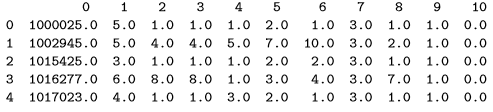
\includegraphics{Annotation 2020-03-23 185932.png}
\end{figure}
\paragraph{Normalización.}
Aplicamos normalización maxmin para mejorar el rendimiento y evitar que la columna con valores más altos monopolice el modelo. 
\begin{lstlisting}
names = df.columns[0:10]
scaler = MinMaxScaler() 
scaled_df = scaler.fit_transform(df.iloc[:,0:10]) 
scaled_df = pd.DataFrame(scaled_df, columns=names)
scaled_df[10]= df[10]
\end{lstlisting}
\paragraph{Separar los datos.}
En este ejercicio separamos los datos en 2 sets, el de entrenamiento y el de test. Aprovechamos la versatilidad de la librería pandas para quitar la primera columna, pues el ID del paciente no influye en nada. Trasponemos los datos para que el fichero NeuralNetwork.py pueda trabajar con ellos.
\begin{lstlisting}
x=scaled_df.iloc[0:500,1:10].values.transpose()#500 para train
y=df.iloc[0:500,10:].values.transpose()
xval=scaled_df.iloc[501:683,1:10].values.transpose()
yval=df.iloc[501:683,10:].values.transpose()#168 para el tets
\end{lstlisting}
\paragraph{Implementación de la red.}
En este apartado hacemos uso de las funciones de NeuralNetwork.py, la razón de desarrollar dicho fichero fue poder implementar redes neuronales de forma sencilla y poder aplicarla en distintos problemas sin tener que programar lo mismo otra vez. Ahora lo vemos en práctica.\\
Declaramos la red neuronal con los valores de entrenamiento y un learning rate de 0.01. La red funciona con una arquitectura [9 - 15 - 1], la cual utiliza funciones de salida lineales en la capa intermedia y una sigmoidal en la de salida. Utiliza como función de error, en lugar del clásico MSE, el Cross-Entropy. \\El algoritmo de aprendizaje utilizado es el descenso por gradiente, el cual implementa el algoritmo de backpropagation.\\
Tanto la arquitectura como el learning rate son valores que hemos definido basándonos en la experiencia, en el anexo se muestran diversas implementaciones que nos han llevado a elegir la mejor.
\begin{lstlisting}
nn = NeuralNetwork(x,y,0.01,0)
nn.gradient_descent(50000)
\end{lstlisting}
\begin{figure}[H]
\centering
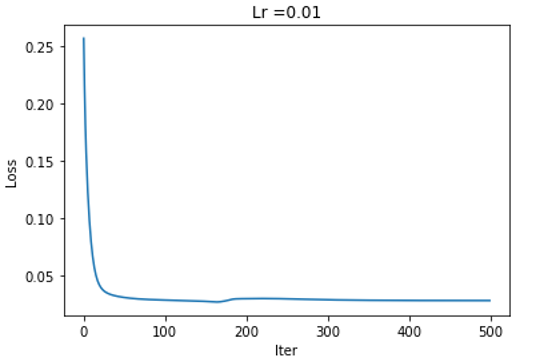
\includegraphics[scale=0.6]{Annotation 2020-03-23 190119.png}
\end{figure}

Imprimimos los resultados, nótese que este modelo no usa regularización.
\begin{lstlisting}
pred_train = nn.predict(x, y)
pred_test = nn.predict(xval, yval)
Acc: 0.9240000000000003
Acc: 0.9835164835164836
\end{lstlisting}
\paragraph{Con regularización.}
Tras diversas pruebas, el valor 0.7 es el que mejor rendimiento consigue. Elevando el acierto en el test al máximo.
\begin{lstlisting}
pred_train = nn.predict(x, y)
pred_test = nn.predict(xval, yval)
Acc: 0.9360000000000003
Acc: 1.0
\end{lstlisting}
\subsubsection{Visualización.}
Para visualizar los datos de forma más explicativa se ha recurrido a una matriz de confusión que muestra el número de positivos clasificados correctamente, falsos positivos, falsos negativos, y  negativos clasificados correctamente. La función es la siguiente:
\begin{lstlisting}
def plotCf(a,b,t):
    cf =confusion_matrix(a,b)
    plt.imshow(cf,cmap=plt.cm.Blues,interpolation='nearest')
    plt.colorbar()
    plt.title(t)
    plt.xlabel('0         Predicted         1')
    plt.ylabel('1          Actual            0')
    tick_marks = np.arange(len(set(a))) # length of classes
    class_labels = ['0','1']
    plt.xticks(np.ndarray([0,1]))
    plt.yticks(np.ndarray([0,1]))
    for i,j in itertools.product(range(cf.shape[0]),range(cf.shape[1])):
        plt.text(j,i,format(cf[i,j],'d'),horizontalalignment='center',
           color='white' if cf[i,j] > (cf.max()*0.7) else 'black')
    plt.show();
\end{lstlisting}
Aquí podemos aplicar el umbral que deseamos, como estamos hablando de un tema tan sensible como el cáncer, nuestro umbral debe ser alto para solo afirmar en caso de mucha certeza.

\begin{lstlisting}
nn.X,nn.Y=xval, yval 
target=np.around(np.squeeze(yval), decimals=0).astype(np.int)
predicted=np.around(np.squeeze(nn.predict(xval,yval)), decimals=0)
plotCf(target,predicted,'Cf Validation Set')
\end{lstlisting}
\begin{figure}[H]
\centering
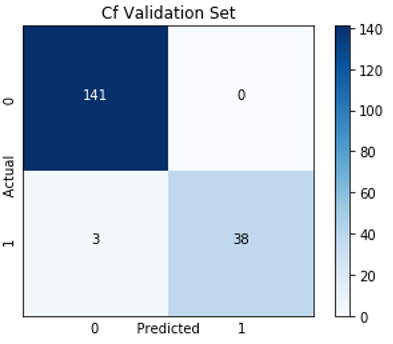
\includegraphics[scale=0.6]{Annotation 2020-03-23 190419}
\end{figure}
El modelo, incluso sin regularización, muestra un resultado excelente. Solo hemos clasificado 3 correos mal, todos eran spam y los hemos clasificado como correos ordinarios.

\subsubsection{Implementación con regresión logística.}
Con el fin de comprobar si un modelo más rápido y sencillo podría superar al ya explicado, hemos implementado regresión logística. Como era de esperar, la regresión logística no es adecuada para tratar problemas de esta emvergadura.
\begin{figure}[H]
\centering
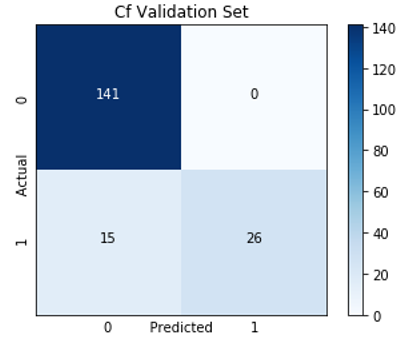
\includegraphics[scale=0.6]{Annotation 2020-03-23 193133.png}
\end{figure}

\subsection{Ejercicio de clasificación de correo electrónico.}
Al igual que en la sección anterior, este ejercicio implementa las funciones definidas en el archivo NeuralNetwork.py.\\ En este caso el ejercicio exige un enfoque ligeramente diferente respecto al anterior a causa de los datos. Los datos utilizados son numerosos mensajes, los cuales algunos son spam y otros mensajes corrientes. \\De dichos mensajes solo se pueden extraer sus palabras, así que, en este caso, no tenemos distintas características que evaluar.


\subsubsection{Carga, comprensión y transformación de los datos.}
Como ya hemos dicho, el dataset está compuesto por frases y su correspondiente etiqueta, hay tres columnas vacías que quitamos.
\begin{lstlisting}
import pandas as pd
import numpy as np
import re
raw = pd.read_csv('spam.csv', delimiter = ',')
raw.head()
\end{lstlisting}
\begin{figure}[H]
\centering
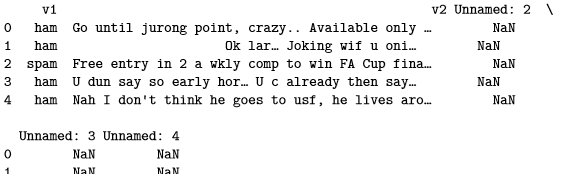
\includegraphics[scale=0.9]{Annotation 2020-03-23 174228.png}
\end{figure}
\begin{lstlisting}
raw.drop(['Unnamed: 2' ,'Unnamed: 3' ,'Unnamed: 4'], axis=1)
raw = raw.dropna(how='any',axis=0)# drop Nan rows
raw.head()
\end{lstlisting}
\begin{figure}[H]
\centering
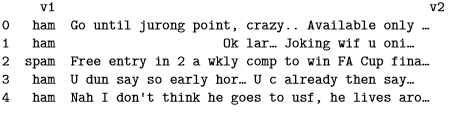
\includegraphics{Annotation 2020-03-23 174341.png}
\end{figure}
Como ya hemos comentado, la única información que podemos extraer de los datos son palabras, en total hay aproximadamente 1000. Como no es viable desarrollar en nuestro equipo una red neuronal con 10000 valores en la capa de entrada, debemos sesgar cuáles queremos.\\ En este caso hemos elegido 100, las 100 que más se repiten. Nótese que con intención de hacer un modelo más eficiente, se podrían considerar otros criterios a parte de la frecuencia de aparición en el dataset.\\
Contamos las palabras:
\begin{lstlisting}
columns=[] 
rows = [] 
y = list(raw.v1)#lo usaremos luego 
for i in range (0,len(raw.v2)): 
    try:
         rows.append(re.sub("[^\w]", " ", raw.v2[i]).lower().split()) 
         columns = columns + re.sub("[^\w]", " ", raw.v2[i]).lower()
    except: 
        print('Error in:' ,raw.v2[i])
from collections import Counter 
    counts = Counter(columns)

    print(counts)
\end{lstlisting}
\begin{figure}[H]
\centering
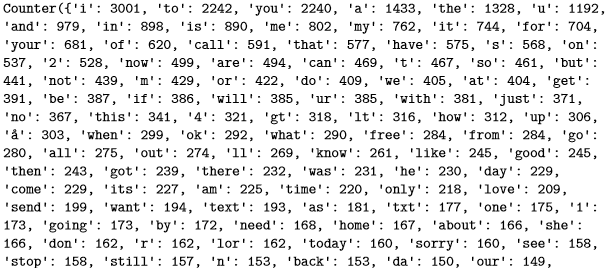
\includegraphics[scale=0.83]{Annotation 2020-03-23 182424.png}
\end{figure}
Elegimos las palabras:
\begin{lstlisting}
columns = list(dict.fromkeys(columns))#delete repeated values 
counts_list = [key for key, _ in counts.most_common()] 
df_columns = counts_list[0:100] 
df_columns.append('y') 
print(df_columns)
\end{lstlisting}

\paragraph{Transformar la información.}
Ahora lo relevante es determinar cómo vamos a introducir la información en la red. Las redes neuronales no aceptan otra entrada que no sea de carácter numérico, eso nos lleva a transformar nuestro set de datos, utilizaremos un 1 cuando la palabra de la frase sea una de las palabras elegidas como entrada de la red y 0 cuando en caso contrario.
\begin{lstlisting}
binary_rows = np.zeros((len(rows),len(df_columns)),dtype=int) 
for i in range(0, len(rows)): 
    for k in range(0,len(rows[i])):
        if rows[i][k] in df_columns: 
	    binary_rows[i][df_columns.index(rows[i][k])]=1
         if k == (len(rows[i])-1) and y[i]=='spam':#if spam=>1 
            binary_rows[i][100]=1
print(binary_rows[2])
\end{lstlisting}
\begin{figure}[H]
\centering
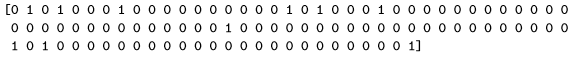
\includegraphics[scale=0.83]{Annotation 2020-03-23 182035.png}
\end{figure}
Creamos un dataframe nuevo con las frases cargadas como secuencias binarias.
\begin{lstlisting}
dataframe = pd.DataFrame(binary_rows,columns=df_columns) 
dataframe.head(5)
\end{lstlisting}
\begin{figure}[H]
\centering
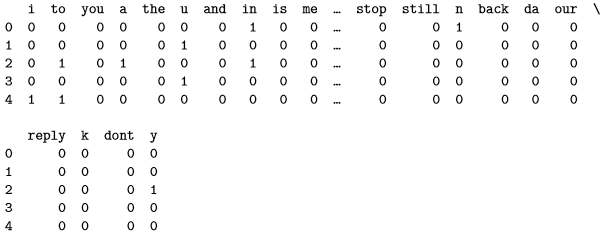
\includegraphics[scale=0.83]{Annotation 2020-03-23 182154.png}
\end{figure}
Por último, creamos los datos en listas para imputarlos posteriormente en la red.
\begin{lstlisting}
Y = (dataframe.y).to_numpy() 
dataframe.drop(['y'], axis=1, inplace=True)
X = dataframe.to_numpy().T 
size = int(X.shape[1] * 0.70) 
x_train, x_test = X[:,0:size], X[:,size:] 
y_train, y_test = Y[0:size], Y[size:]
\end{lstlisting}
\subsubsection{Implementación de la red.}
De nuevo utilizamos el fichero NeuralNetwork.py, en este caso, la  arquitectura  que mejor rendimiento muestra es la 100-25-1, 25 neuronas en una única capa oculta y un ratio de aprendizaje (learning rate) de 0.2. Diversas arquitecturas pueden contrastarse en el anexo de este trabajo.
\begin{lstlisting}
from NeuralNetwork import * 
nn = NeuralNetwork(x_train,y_train,0.02,[100,25,1],0)
nn.gradient_descent(5000)#gradient descent algorithm
\end{lstlisting}
\begin{figure}[H]
	\centering
	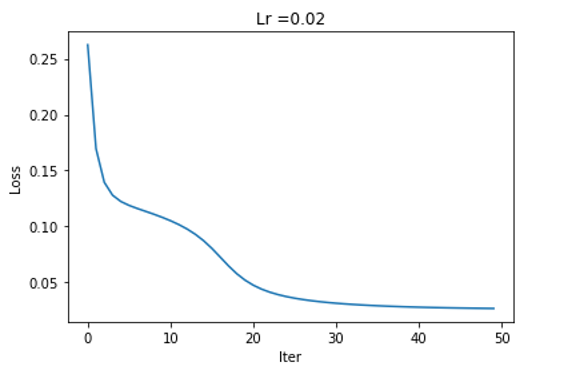
\includegraphics[width=10.0cm,height=7cm]{Annotation 2020-03-23171823}
\end{figure}
\subsubsection{Visualización.}
Implementamos de nuevo la función de la matriz de confusión. La función es la siguiente:
\begin{lstlisting}
def plotCf(a,b,t):
    cf =confusion_matrix(a,b)
    plt.imshow(cf,cmap=plt.cm.Blues,interpolation='nearest')
    plt.colorbar()
    plt.title(t)
    plt.xlabel('0         Predicted         1')
    plt.ylabel('1          Actual            0')
    tick_marks = np.arange(len(set(a))) # length of classes
    class_labels = ['0','1']
    plt.xticks(np.ndarray([0,1]))
    plt.yticks(np.ndarray([0,1]))
    for i,j in itertools.product(range(cf.shape[0]),range(cf.shape[1])):
        plt.text(j,i,format(cf[i,j],'d'),horizontalalignment='center',    
	   color='white' if cf[i,j] > (cf.max()*0.7) else 'black')
    plt.show();
\end{lstlisting}
Llamamos de nuevo a la función. Observamos que esta vez el rendimiento está al rededor del 95 por ciento.
\begin{lstlisting}
nn.X,nn.Y=x_test, y_test 
target= nn.Y
predicted=nn.predict(x_test,y_test) 
plotCf(target,predicted[0],'Cf Validation Set')
\end{lstlisting}
\begin{figure}[H]
\centering
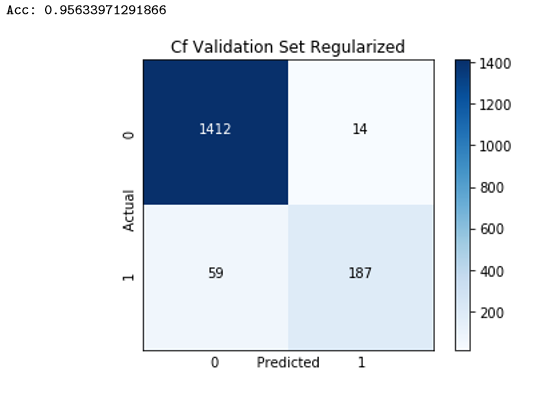
\includegraphics[scale=0.6]{Annotation 2020-03-23 161410}
\end{figure}
Hemos fallado 63 mensajes, de los cuales, 14 han sido clasificado erróneamente como spam y 59 como spam
\subsubsection{Con regularización.}
En este caso la regularización no aporta nada, este método ha sido evaluado con distintos valores, pero ninguna prueba ha aportado ninguna mejora. Teniendo en cuenta esto, es posible que el anterior resultado sea el correspondiente al alcanzar el mínimo absoluto en la función de error.

\subsubsection{Implementación con regresión logística.}
Como podemos observar, en este caso la regresión logística es igual de efectiva que la red neuronal, esto es otra indicación que podemos haber hallado el mínimo absoluto de la función de error.
\begin{lstlisting}
logistic_regression= LogisticRegression()
logistic_regression.fit(x_train.T,y_train)
threshold = 0.5
y_pred = np.where(logistic_regression.predict_proba(x_train.T)[:,1]
					 > threshold, 1, 0)
plotCf(target,y_pred,'Cf Validation Set Logistic Regression')
\end{lstlisting}
\begin{figure}[H]
\centering
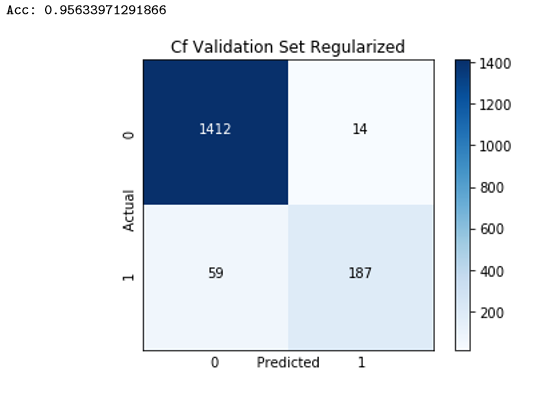
\includegraphics[scale=0.6]{Annotation 2020-03-23 161410}
\end{figure}
\newpage
\subsection{Visión Artificial.}
La visión humana es un sistema muy complejo y poderoso. Simplemente
visualizando una fotografía, el sistema visual humano es capaz
de percibir y definir una gran cantidad de información acerca de ella. Por ejemplo, con la fotografía mostrada, podemos interpretar una inmensa variedad de tonos y colores deducidos del efecto de la luz incidiendo en los pétalos de la flor.
\\Gracias al proceso de detección que realiza el ojo humano, podemos reconocer figuras, bordes, contornos, etc., podemos incluso segmentar la flor del resto de la imagen e interpretar factores como la profundidad a pesar de estar viendo una imagen en dos dimensiones (virtualmente).\\
El proceso seguido para ello consta de dos partes:
\begin{itemize}
\item Por un lado, la luz reflejada por los objetos llega hasta nuestros ojos, formándose en la retina una imagen invertida en dos
dimensiones. 
\item Por otro lado, dicha imagen es transformada en impulsos nerviosos y trasladada a la parte posterior de cerebro, 
el cual reconstruye un modelo en tres dimensiones de la imagen, gracias a la intervención de millones de neuronas. Al mismo tiempo nuestro cerebro asocia la imagen con el concepto previamente asimilado de lo que es de una flor y la reconoce como tal.
\end{itemize}

\begin{figure}[H]
\centering
\includegraphics[width=8.5cm, height=5.35cm]{flor.jpg}
\end{figure}
\noindent
La Visión Artificial, conocida también como visión por computador, es la disciplina que trata de otorgar a los ordenadores la capacidad de percibir, procesar  e interpretar imágenes de forma análoga a la visión humana. \\Nótese que el ordenador percibe imágenes como matrices de valores numéricos, típicamente comprendidos en el rango de 0 a 255. En el caso de las imágenes RGB este rango se mantiene, pero se amplia la cantidad de información a tres matrices, una por color.\\
En las siguientes subsecciones veremos las aplicaciones más comunes de la visión artificial, además de explicar sus limitaciones.

\subsubsection{Aplicaciones.}
En la actualidad existe una gran variedad de aplicaciones de la visión artificial, es una ciencia que está presente en muchísimos campos. Los más comunes son:
\begin{itemize}
\item Reconocimiento óptico de caracteres (OCR): esta técnica consiste en la lectura e identificación de los caracteres alfanuméricos de una imagen.\\ A día de hoy está considerado un problema sencillo de resolver. Su primera aplicación data de los años 60, y fue empleado en el reconocimiento de códigos postales por el servicio de correo de Estados Unidos.
\begin{figure}[H]
\centering
\includegraphics[scale=0.7]{ocr.jpg}
\end{figure}
\item Construcción de modelos 3D (fotogrametría): esta técnica se basa en la construcción de figuras 3D mediante imágenes 2D.
\begin{figure}[H]
\centering
\includegraphics[scale=0.4]{fotogrametria-png.png}
\end{figure}
\item Monitorización: La capacidad de reconocer cualquier objeto captado por la cámara da lugar a multitud de aplicaciones. \\Un claro ejemplo se puede ver en la vigilancia de carreteras. En la actualidad existen sistemas para detectar accidentes de tráfico en el momento en el que sucede.
\begin{figure}[H]
\centering
\includegraphics[width=10.5cm, height=4cm]{cars.png}
\end{figure}
\item Medicina: la medicina es uno de los campos que más partido saca de la visión artificial. Un ejemplo es la detección automática de melanomas.
\item Conducción autómata: la conducción autómata es uno de los campos más investigados actualmente. Empresas como Tesla están a la cabeza en la investigación sobre este tema. \\A día de hoy, ya es posible circular en un vehículo que conduce solo por vías fuera de poblado.
\begin{figure}[H]
\centering
\includegraphics[width=6.5cm, height=4.5cm]{melanoma.jpg}\hfill
\includegraphics[width=6.5cm, height=4.5cm]{cars.jpg}
\end{figure}
\end{itemize}

\subsubsection{Problemas y limitaciones de la Visión Artificial.}
El rendimiento de los algoritmos de Visión Artificial está drásticamente ligado a la calidad de los datos. Es mucho más difícil adquirir un buen set de datos cuando hablamos de imágenes que en el caso de otras ramas del Machine Learning.
\\Aunque existen técnicas de filtrado digital es frecuente encontrarse con limitaciones que dificultan el trabajo de los profesionales. Estas son:
\begin{itemize}
\item Variaciones en el punto de vista: es frecuente encontrarse en los conjuntos de imágenes que han sido tomadas desde diferentes tipos de vista. \\En ocasiones, como en la conducción automática, esto es inevitable y tratar con ello es parte de la tarea de desarrollo. Pero este problema también se presenta en campos como en la medicina, donde no hay una razón aparente que justifique esta inconveniencia. 
\item Variaciones de escala: es frecuente encontrar imágenes con distintos tamaños, bien por la posición desde donde se han tomado o por las cámaras que se han usado.
\item Variación lumínica: una variación en la luz puede cambiar drásticamente los valores de una imagen: Recordemos que una imagen es interpretada como una matriz de píxeles por el ordenador.
\item Oclusión:  un objeto puede estar oculto parcialmente en la imagen. Por ejemplo, un peatón que otro coche tapa parcialmente.
\item Ruido inherente: existen matices frecuentes en algunas fotografías que dificultan mucho el tratamiento de estas. Por ejemplo, la presencia del cabello del paciente en una foto de su lunar.

\end{itemize}



\newpage
\subsection{Redes convolucionales.}
En este apartado explicaremos las redes neuronales que vamos a necesitar para implementar el último ejercicio del trabajo; estas son las redes convolucionales, en adelante CNN. \\Las CNN se utilizan en problemas de clasificación de imágenes como alternativa al tipo de red que ya hemos visto, pues este queda obsoleto ante una gran cantidad de datos en la capa de entrada, como es en el caso de las imágenes.\\ Procedemos a explicar las novedades y conceptos que dicha red incorpora.\\

\subsubsection{Filtros.}
Los filtros son matrices de tamaño configurable, siempre menores que la matriz de entrada, estos se aplican por toda la imagen. El resultado es una nueva matriz cuyos datos derivan de los productos matriciales del filtro y la fotografía. Estos filtros son capaces de extraer características como líneas, curvas, contornos, etc.  \\Es decir, si aplicamos un filtro para las líneas verticales y otro para las horizontales, el resultado serán dos imágenes, cada una solo con la información para la que hemos aplicado el filtro.
\begin{figure}[H]
\centering
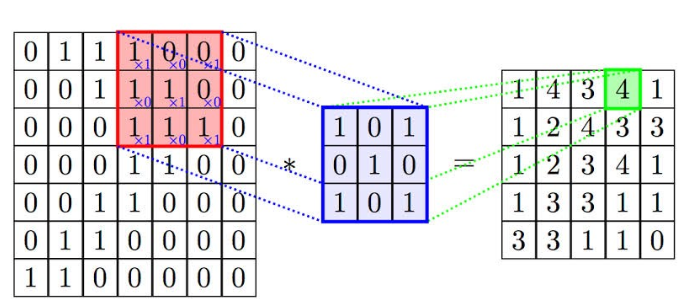
\includegraphics[width=12.0cm, height=4.5cm]{Annotation 2020-04-13 191448.png}
\end{figure}
\noindent
Si lo comparamos con una ANN, los filtros son los pesos que se entrenan. De esta forma, comenzando con filtros aleatorios, estos se modifican hasta ser los más adecuados para procesar y clasificar las imágenes que conciernen.\\
Hay tres parámetros imprescindibles a la hora de definir un filtro:
\begin{itemize}
\item Tamaño: podemos definir el tamaño del filtro, que varía en función del tamaño de la imagen y de las características que nos gustaría extraer.  Normalmente se utilizan matrices. cuadradas
\item Stride:  es el intervalo de posiciones en el que aplicamos el filtro. Si nuestro filtro tiene un stride de 1, el filtro se desplazará por la imagen de píxel en píxel,  si ponemos el valor a dos, lo hará de dos píxeles en dos píxeles. Es decir, se aplicará el filtro cubriendo todos los valores de la imagen, pero el centro del filtro solo coincidirá con la mitad los datos de la imagen. 
\item Padding: es evidente que al aplicar un filtro no es posible que este recorra la matriz de forma equitativa independientemente del stride. Por ejemplo, en caso de los datos de las esquinas solo se les aplicaría una vez según la explicación dada. El padding indica un margen adicional que introducimos con valores de cero alrededor de la matriz para permitir aplicar el filtro por la totalidad de la imagen. \\Existen dos tipos de padding:
	\begin{itemize}
	\item Valid: implica que no hay padding, lo que hace que se pierda información de los contornos de la imagen.\begin{figure}[H]
\centering
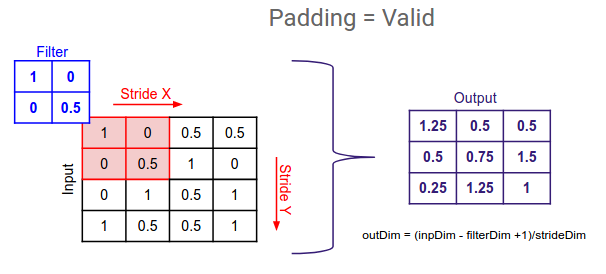
\includegraphics[width=10.0cm, height=4.5cm]{Annotation 2020-04-13 214927.png}
\end{figure}
	\item Same: incluye tantas como sea necesario para que el tamaño de la salida sea igual al de entrada.\begin{figure}[H]
\centering
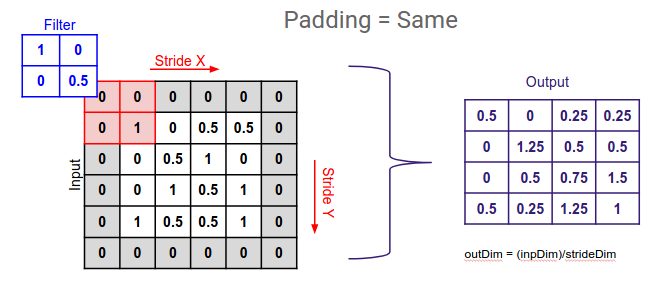
\includegraphics[width=11.0cm, height=4.5cm]{Annotation 2020-04-13 215118.png}
\end{figure}
	\end{itemize}
\end{itemize}
Estos factores son los que determinan el tamaño de la matriz de salida (n), siendo el tamaño del filtro (f), el de la matriz de entrada (i), padding (p) y stride(s).
\[
n=\frac{i+2p-f}{s}  +1
\]


\subsubsection{Capa convolucional.}
Las capas convolucionales son el núcleo de las CNN, son las capas de la arquitectura donde se aplica la operación de convolución. \\La operación consiste en desplazar el filtro por la matriz, aplicándolo en cada dato hasta cubrirla completamente. En cada desplazamiento se realiza un producto matricial. Dicho proceso se repite tantas veces como números de filtros hayamos dispuesto en nuestra capa convolucional (k), de forma que si hemos dispuesto 32 filtros para una imagen de 28*28 píxeles, la salida será de 28*28*32 = 25.088 píxeles.
 \\La siguiente fórmula muestra cómo se calcula el número de datos correspondiente a la salida de la capa convolucional.

\[
n=\frac{i+2p-f}{s}  +1
\]
\[
output = k * n
\]

Normalmente, tras la capa de convolución, todas las salidas son procesadas por una función ReLu.\\
A primera vista puede parecer que 25.088 datos para una foto tan simple resultan algo disparatado, pero si nos planteamos la cantidad de datos que habría en una red neuronal convencional, no lo es. \\
Supongamos que tenemos la misma imagen, pero en lugar de una capa convolucional, implementamos una capa con el mismo número de neuronas que el de la capa de entrada. Si cada entrada está conectada a todas las neuronas de la capa siguiente (característica bastante frecuente), el resultado del número de datos sería el cuadrado de la entrada, es decir, 614.656 datos, solo para abordar los pesos. \\
Aún con esta ventaja, las CNN cuentan con otro mecanismo para aligerar la carga de información.


\subsubsection{La capa de pooling.}
Esta es la capa que se encarga de realizar la reducción del volumen de datos, perdiendo la menor información posible.\\ Supongamos que tenemos el mismo bloque de datos del ejemplo anterior, 25.088 datos en una matriz de 28*28*32. Es evidente que si queremos reducir la dimensionalidad de la matriz, no podemos alterar la dimensión de 32, pues estaríamos quitando filtros que se han añadido en la capa convolucional.\\
Existen dos tipos de pooling:
\begin{itemize}
\item Max pooling: consiste en reducir las dimensiones de una matriz, separándola en subconjuntos de tamaño configurable y conservando solo el valor mayor de cada fragmento. Dichos subconjuntos se hacen sigiuendo el mismo criterio que seguimos para desplazar los filtros, de forma que, a mayor stride, más se reducirá la matriz.
\begin{figure}[H]
\centering
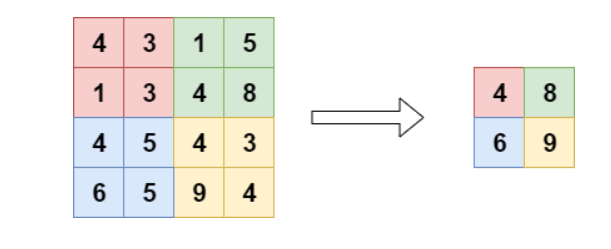
\includegraphics[width=11.0cm, height=4.5cm]{maxpool.png}
\end{figure}
\item Mean pooling: el proceso es análogo al maxpooling, solo que en esta ocasión, el valor conservado es el medio de los subconjuntos.
\begin{figure}[H]
\centering
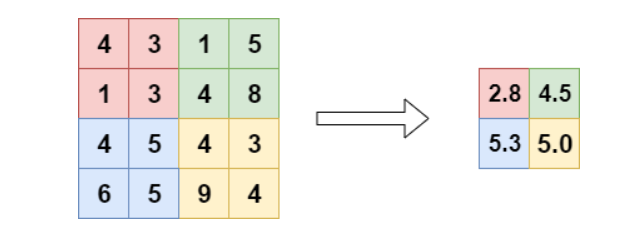
\includegraphics[width=11.0cm, height=4.5cm]{meanpool.png}
\end{figure}
\end{itemize}

\subsubsection{Capa totalmente conectada y red neuronal.}
Esta capa, también conocida como flatten, es una capa a la que se conectan a todas las salidas de la capa anterior (convolucional o de pooling) con una capa con tantas neuronas como datos. Posteriormente se realiza una arquitectura con una o dos capas intermedias y una capa de salida con tantas neuronas como clases tenga nuestro problema de clasificación. En estas capas puede aplicarse regularización.
\subsubsection{Regularización Dropout.}
Aunque este tipo de regularización no es exclusiva de las CNN, la regularización dropout nos será de gran utilidad en la práctica. \\Esta consiste en desechar aleatoriamente el porcentaje indicado de pesos de una capa en concreto. Dichos pesos ignorados, serán diferentes en cada iteración del entrenamiento, dejando al azar cuales lo son de forma consecutiva y cuales no.\\ Este método, aunque pueda parecer algo tosco, es una herramienta muy utilizada en algunos campos del Machine Learning y su eficacia ha sido ampliamente probada.
\subsubsection{Arquitecturas.}
En el desarrollo de la CNN, podemos usar nuestros conocimientos teóricos para programar, pero existen ciertas redes muy conocidas que han demostrado en numerosos problemas un buen rendimiento. En la práctica intentaremos imitar la arquitectura de dichas redes.
\begin{itemize}
\item LeNet: es una red neuronal desarrollada por Yann LeCun en 1998. Su versión más conocida es la arquitectura con cinco capas. \begin{figure}[H]
\centering
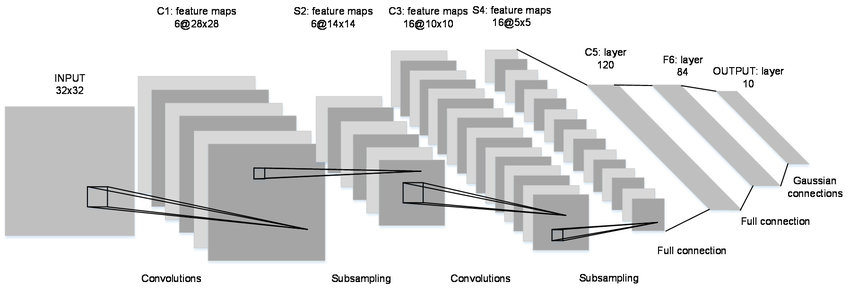
\includegraphics[width=14.0cm, height=4.5cm]{lenet5.png}
\end{figure}
\item AlexNet: desarrollada por Alex Krizhevsky, ganó el concurso ImageNet Large Scale Visual Recognition Challenge en septiembre de 2012. Es una red neuronal muy eficiente pero que conlleva un alto coste computacional debido a su paralelización en dos CNN , es inviable usarla sin GPU.\begin{figure}[H]
\centering
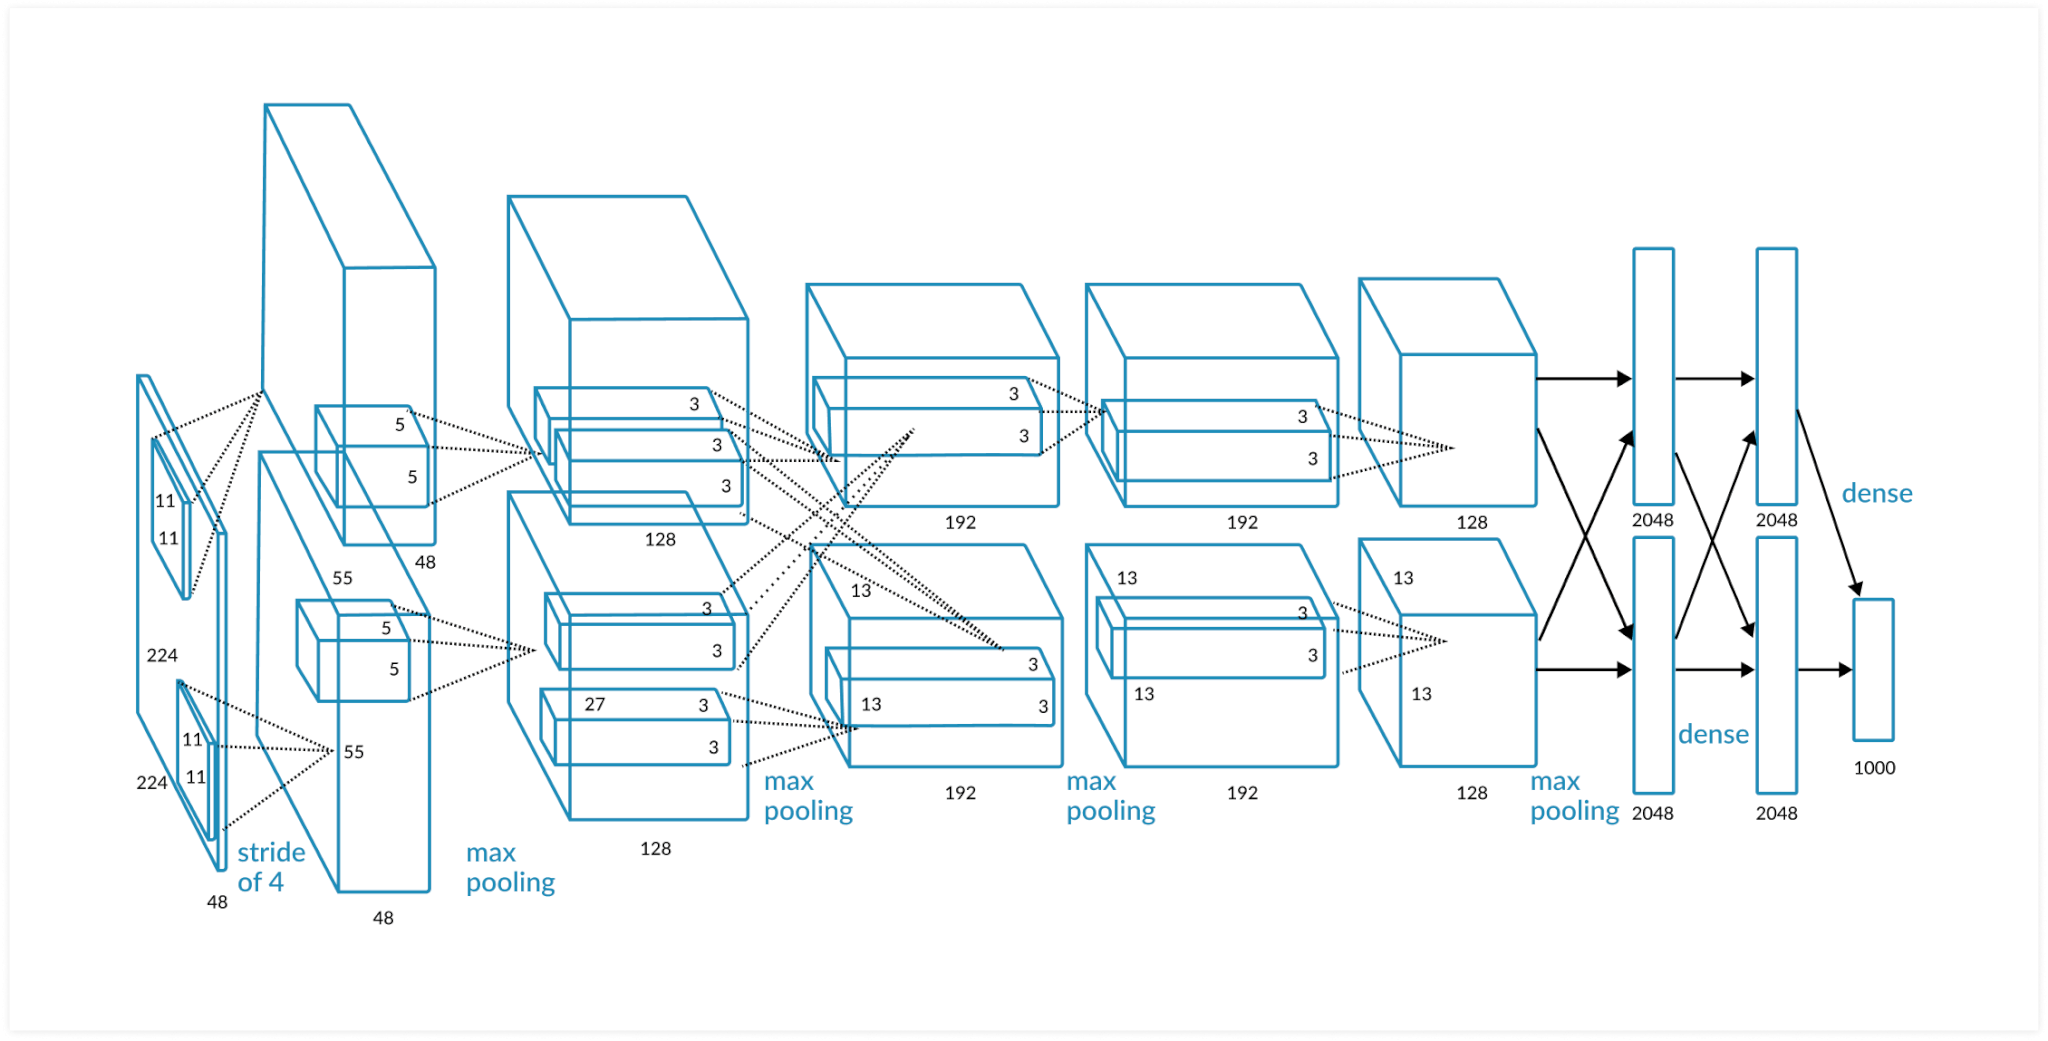
\includegraphics[width=14.0cm, height=4.5cm]{AlexNet2012.png}
\end{figure}
\item VGG16: propuesta por K. Simonyan y A. Zisserman. El modelo alcanzó un 0.927 de precisión en ImageNet, un dataset de 14 millones de imágenes en 1000 clases. \begin{figure}[H]
\centering
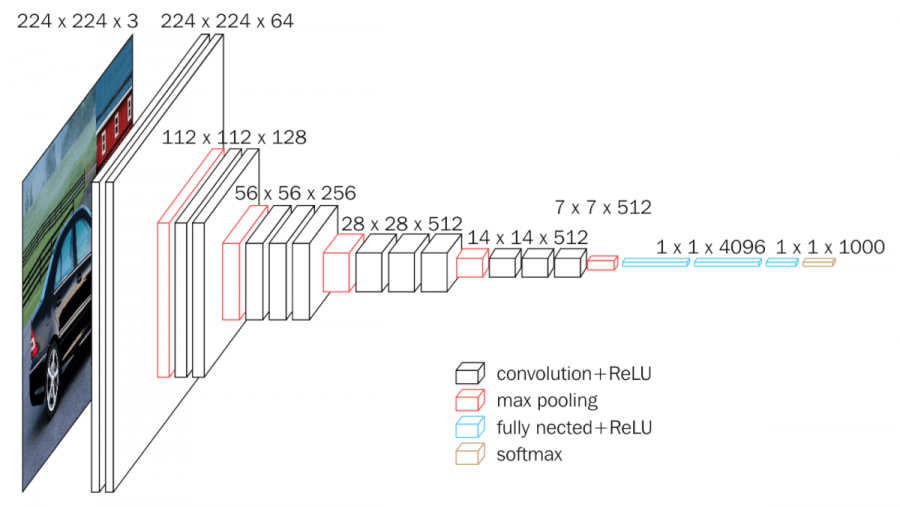
\includegraphics[width=12.0cm, height=4.5cm]{vgg16-1-e1542731207177.png}
\end{figure} 	
\item ResNet: desarrollada por Microsoft en 2015, también ganó el ImageNet Large Scale Visual Recognition Challenge. Tiene varias configuraciones: con 50, 101 y 152 capas.\begin{figure}[H]
\centering
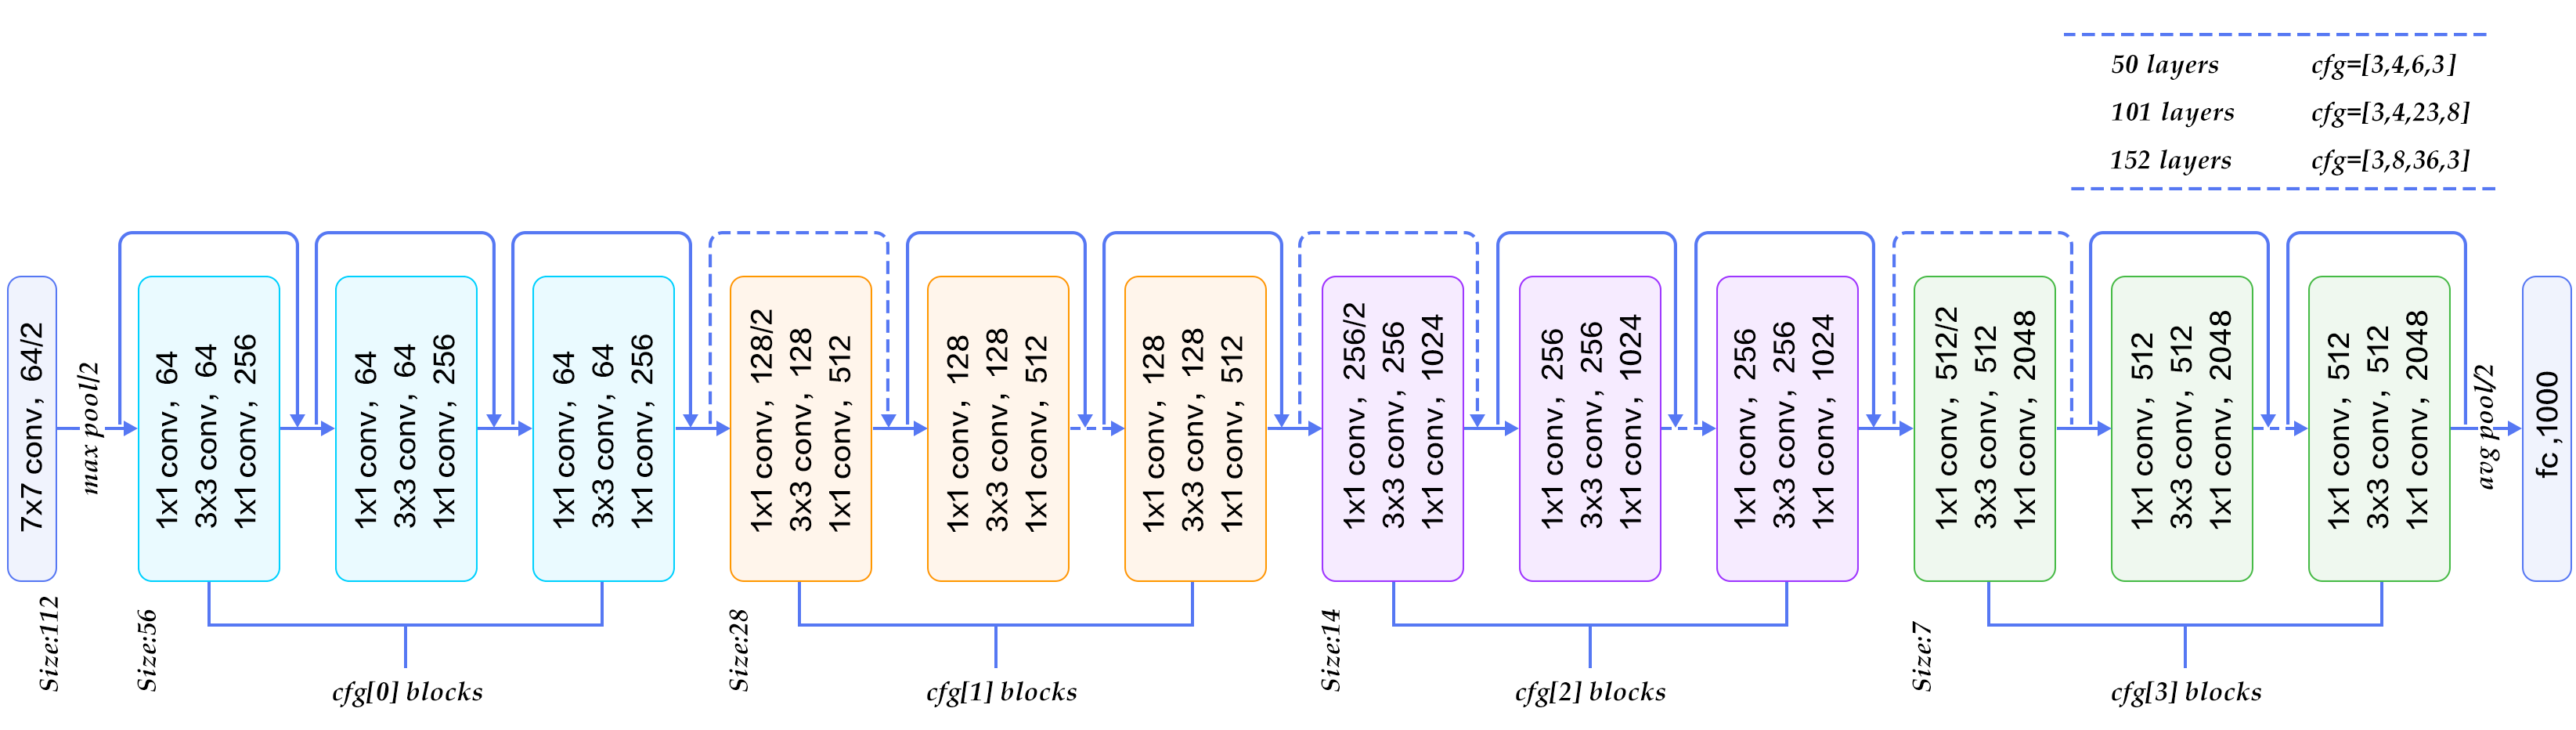
\includegraphics[width=12.0cm, height=4.5cm]{resnet.png}
\end{figure} 	
\end{itemize}

\newpage

\subsection{Aplicación práctica: Clasificación de señales de tráfico.}
En el siguiente ejercicio vamos a clasificar 43 tipos de imágenes de señales de tráfico en python mediante una CNN. \\
El set de datos que utilizaremos contiene 32902 imágenes divididas en carpetas en función del tipo para el entrenamiento y 12630 para la prueba.
\subsubsection{Carga de los datos.}
En esta ocasión los datos de entrenamiento y prueba están almacenados de distinta forma, por ello es necesario que implementemos dos funciones para realizar la carga.
\paragraph{Carga de datos de entrenamiento.}
Los datos de entrenamiento están almacenados dentro en 43 carpetas dentro de la carpeta "Train". Debemos recorrer dicho directorio, importar las imágenes RGB y transformarlas en un array de cara a poder manejarlas posteriormente.\\
Como no todas las fotos presentan el mismo tamaño, modificamos ligeramente sus dimensiones con el fin de trabajar siempre con matrices del mismo tamaño, en este caso de 30*30.\\
Determinaremos la clase de cada imagen en el momento de carga basándonos en la carpeta en la que se encuentre. \\Una vez realizada la carga, devolvemos las imágenes y su clase en formato de matriz.
\begin{lstlisting}
def load_train(folders,size):
    X=[]
    Y=[]
    for i in range(folders) :
        path = "ruta al directorio principal"
        folder=os.listdir(path)
        for img in folder:
            try:
                image=cv2.imread(path+img)
                image_RGB = Image.fromarray(image, 'RGB')
                resized_image = image_RGB.resize(size)
                X.append(np.array(resized_image))
                Y.append(i)
            except AttributeError:
                print("Error loading picture ", img)
    return np.asarray(X),np.asarray(Y)
\end{lstlisting}

\paragraph{Carga de datos de prueba.}
Esta función carga los datos de prueba. A diferencia de en el apartado anterior, la clase de cada foto se extrae de un archivo csv de con los metadatos. En el resto de la función es como igual a la utilizada en la carga de datos.

\begin{lstlisting}
def load_train(folders,size):
    X=[]
    Y=[]
    for i in range(folders) :
        path = "ruta al directorio principal"
        folder=os.listdir(path)
        for img in folder:
            try:
                image=cv2.imread(path+img)
                image_RGB = Image.fromarray(image, 'RGB')
                resized_image = image_RGB.resize(size)
                X.append(np.array(resized_image))
                Y.append(i)
            except AttributeError:
                print("Error loading picture ", img)
    return np.asarray(X),np.asarray(Y)
\end{lstlisting}

\subsubsection{Manipulación de los datos.}
Tras cargar los datos debemos mezclar los datos. El modelo debe tener las imágenes barajadas para no ir entrenando clase por clase, esto afecta drásticamente al rendimiento. \\
También creamos un set de datos de validación del 20\% del volumen total de entrenamiento para estudiar la evolución del entrenamiento en tiempo real.
\begin{lstlisting}
X,Y=load_train(43,[30,30])
#shuffle the data
s=np.arange(X.shape[0])
np.random.seed(43)
np.random.shuffle(s)
X=X[s]
Y=Y[s]
#Spliting the images 
(X_train,X_val)=X[(int)(0.2*len(Y)):],X[:(int)(0.2*len(Y))]
X_train = X_train.astype('float32')/255 #Train normalization 
X_val = X_val.astype('float32')/255 #Test normalization
(y_train,y_val)=Y[(int)(0.2*len(Y)):],Y[:(int)(0.2*len(Y))]
\end{lstlisting}
Imprimimos la simágenes a tratar:
\begin{lstlisting}
fig=plt.figure(figsize=(10,10))
img=[]
for i in range(1, 13):
    ax = fig.add_subplot(3, 4, i)
    ax.title.set_text('Senal {0}'.format(i))
    plt.imshow(X_train[i][:, :, [2, 1, 0]], interpolation='nearest')
plt.show()
\end{lstlisting}
\begin{figure}[H]
\centering
\includegraphics[scale=0.8]{Annotation 2020-04-28 121743.png}

\end{figure}


\subsubsection{Arquitectura.}
La arquitectura escogida es una versión simplificada que al modelo VGG16. La arquitectura es la siguiente.
\begin{itemize}
\item Capa convolucional: 32 filtros de tamaño 5*5, stride de 1 y valid para el padding.
\item Capa convolucional: 64 filtros de tamaño 3*3, stride de 1 y valid para el padding.
\item Capa maxpooling: tamaño de 2,2 con stride de 1 y valid para el padding.
\item Capa de dropout del 25\%: descartamos el 25\% de los datos aleatoriamente para prevenir overfitting.
\item Capa convolucional: 64 filtros de tamaño 3*3, stride de 1 y valid para el padding.
\item Capa maxpooling: tamaño de 2,2 con stride de 1 y valid para el padding.
\item Capa de dropout del 25\%.
\item Capa fully-connected.
\item Capa de 256 neuronas.
\item Capa de dropout del 50\%.
\item Capa de salida, 43 neuronas con la función softmax.
\end{itemize}
Los elementos de la arquitectura han sido elegidos como resultado del estudio de la materia mostrada y se han ido ajustando en función de los resultados obtenidos durante el desarrollo. Las principales razones son:
\begin{itemize}
\item Debido al tamaño de las fotos los filtros no sobrepasan el tamaño de 5. 
\item Dado que en todas las fotografías las señales no se ajustan a los bordes, los píxeles que forman el contorno de la imagen no aportan información respecto a la naturaleza de la señal, es por ello que hemos decidido establecer el padding como valid.
\item Por otro lado, la razón de que el stride sea igual a 1, lo cual supone una bajada de rendimiento como se muestra en la fórmula del apartado X, es que no queremos perder información de imágenes con tan poca cantidad de píxeles.
\end{itemize}

Esta arquitectura se implementa en la siguiente función:
\begin{lstlisting}
def build_model():
    model = Sequential()
    model.add(Conv2D(32, kernel_size=5,padding='valid', strides=1, 
                     activation='relu', input_shape=(30,30,3)))
    model.add(Conv2D(64, kernel_size=3,padding='valid', strides=1,
                     activation='relu'))
    model.add(MaxPooling2D(pool_size=(2, 2), strides=1, padding=
                     'valid', data_format=None))
    model.add(Dropout(0.25))
    model.add(Conv2D(64, kernel_size= 3,padding='same', strides=1, 
                     activation='relu'))
    model.add(MaxPooling2D(pool_size=(2, 2), strides=1, padding=
                      'valid', data_format=None))
    model.add(Dropout(0.25))
    model.add(Flatten())
    model.add(Dense(256, activation='relu')
    model.add(Dropout(rate=0.5))
    model.add(Dense(43, activation='softmax'))
    return model
\end{lstlisting}

\subsubsection{Entrenamiento y resultados.}
Por último, entrenamos la CNN utilizando  la función de error de crross-entropy y el optimizador adam, el cual es una versión mejorada del gradient descent que permite modificar el learning rate durante el entrenamiento. Entrenamos 5 iteraciones.
\begin{lstlisting}
#Compilation of the model
model=build_model()
model.compile(
    loss='categorical_crossentropy', 
    optimizer='adam', 
    metrics=['accuracy']
)
#entrenamos el modelo 55 iteraciones
epochs = 5
history=model.fit(X_train, y_train, batch_size=32, epochs=epochs,
				validation_data=(X_val, y_val))
\end{lstlisting}
\begin{figure}[H]
\centering
\includegraphics[width=6.0cm, height=4.5cm]{Annotation 2020-04-24 115814.png}\hfill
\includegraphics[width=6.0cm, height=4.5cm]{Annotation 2020-04-24 120025.png}
\end{figure}

\noindent
Vemos que la red funciona de forma correcta, con una rápida convergencia de la función de error. Como resultado en el set de prueba, obtenemos una precisión del 96\%.

\begin{lstlisting}
X_test,Y_test=load_test([30,30])
X_test = X_test.astype('float32')/255 
y_pred = model.predict_classes(X_test)

from sklearn.metrics import accuracy_score
print(accuracy_score(Y_test, y_pred))
0.9691211401425178#casi un 97%
\end{lstlisting}


\section{Marco técnico.}
En este apartado cubriremos las herramientas utilizadas en el desarrollo del trabajo. Estas se desglosan en :
\begin{itemize}
\item Lenguaje de programación utilizado.
\item Librerías y bibliotecas adicionales de minería de datos y machine learning que aportan algoritmos ya desarrollados.
\item Entornos  de desarrollo.
\end{itemize}
\subsection{Python.}
Python es un lenguaje de programación	más usado actualmente, destaca por la legibilidad en su código. Su nombre es en honor al grupo británico de cómicos Monty Python, su creador decidió llamarlo así debido a que el lenguaje es "sencillo y divertido".\\
Es un lenguaje interpretado y  multiparadigma, ya que soporta programación orientada objetos, imperativa y funcional. Otro de los grandes puntos a favor es que Python es un lenguaje no tipado.\\
Todas estas características describen una herramienta versátil ideal para este trabajo. 
\subsection{Frameworks y librerías.}
Los frameworks y librerías de Python son la razón de que sea el lenguaje ideal para el desarrollo de inteligencia artificial. Acontinucaión se describen los más usados en este trabajo.
\begin{itemize}
\item Numpy: es la librería utilizada para las operaciones de datos. Permite realizar cálculos tediosos en una sola línea de código. Su mejor faceta reside en las listas de la librería, las cuales pueden ser n-dimensionales.
\item Pandas: es la librería referente en extracción de datos. Durante todo el desarrollo trabajaremos cargando los datos gracias a esta librería y usando constantemente sus dataframes.
\item Matplotlib: librería muy utilizada para visualización de datos. En este trabajo solo utilizaremos un ápice de su potencial.
\item Tensorflow: es el framework que utilizaremos para los modelos. Es un framework de código abierto desarrollado por Google. Permite instanciar redes neuronales, así como configurar sus capas en pocas líneas de código, solo preocupándonos de los parámetros a configurar. En el trabajo usaremos su versión de GPU, la cual utiliza la tarjeta gráfica para procesar la información, agilizando mucho la tarea de entrenamiento del modelo.
\item Keras: es la librería "front end"  de Tensorflow, esto significa que es el intermediario entre nosotros y el propio framework. En el desarrollo, utilizaremos keras pero Tensorflow hará el trabajo  computacional.
\end{itemize}

\subsection{Entornos de desarrollo.}
Los entornos de desarrollo (o IDE's) son las herramientas que nos permiten programar de manera más sencilla y eficaz. A continuación, describimos los utilizados en el trabajo.
\subsubsection{Visual Studio Code.}
Es un entorno creado por Microsoft a caballo entre los entornos clásicos y los editores de texto. No es exclusivo de Python pero aporta multitud de facilidades al desarrollador gracias a su gran cantidad de extensiones.
\subsubsection{Jupyter Notebooks.}
Es uno de los entornos más utilizados en Ciencia de Datos. Tiene dos características que lo hacen ideal para esta área:
\begin{itemize}
\item  Celdas: permite ejecutar el código por celdas o bloques. Esto agiliza mucho el desarrollo, permitiendo realizar la carga de datos una sola vez pero realizar tantas modificaciones como queramos en el modelo.
\item Markdown: en los notebooks podemos implementar celdas en lenguaje Markdown, un lenguaje sencillo que permite añadir explicaciones al código. El resultado es un notebook en el que se explica cada paso y resultado del código de una forma muy intuitiva.
\end{itemize}
\end{document}	



